%-------------------------------------------------------------------------
% info-S1-fonctions.tex
%-------------------------------------------------------------------------

%-------------------------------------------------------------------------
\section{Introduction}
%-------------------------------------------------------------------------

%-------------------------------------------------------------------------
\subsection{Réutiliser}\label{sub:reutiliser}
%-------------------------------------------------------------------------

\marginpar{\footnotesize\em
\begin{rem}
Les chiffres $r_i$ en base $b$ sont tels que $0\leq r_i < b$.\\
Exemples : 

\mbox{}\hfill\begin{minipage}[t]{7cm}
\begin{description}
\item[$b = 2$ :] $r_i \in \{0,1\}$ ({{\em bit} = {\bf bi}nary digi{\bf t}})

\item[$b = 10$ :] $r_i \in \{0,1,2,3,4,5,6,7,8,9\}$

\item[$b = 16$ :] $r_i \in \{0,1,2,3,4,5,6,7,8,9,a,b,c,d,e,f\}$
\end{description}
\end{minipage}\\[2mm]
Plus la base $b$ est faible plus il faut de chiffres pour représenter 
un même nombre.\\
Exemples :

\mbox{}\hfill$\displaystyle\begin{array}{llllr}
(128)_{10} &=& 1.10^2 + 2.10^1 + 8.10^0  &=& (128)_{10}\\
           &=& 1.2^7                     &=& (10000000)_{2}\\
           &=& 8.16^1                    &=& (80)_{16}
\end{array}$
\end{rem}
}
\begin{ex}[Numération en base $b$]\label{ex:numeration}
Un entier positif en base $b$ est représenté par une suite de
chiffres {$(r_nr_{n-1}\ldots r_1r_0)_b$}
où les $r_i$ sont des chiffres de la base $b$ ($0\leq r_i < b$).
Ce nombre a pour valeur:
$$r_nb^n + r_{n-1}b^{n-1} + \ldots + r_1b^1 + r_0b^0 = \sum^{i=n}_{i = 0} r_ib^i$$
Exemples :
$\displaystyle\begin{array}[t]{llllr}
(123)_{10} &=& 1.10^2 + 2.10^1 + 3.10^0  &=& (123)_{10}\\
(123)_{5}  &=& 1.5^2 + 2.5^1 + 3.5^0     &=&  (38)_{10}\\
(123)_{8}  &=& 1.8^2 + 2.8^1 + 3.8^0     &=&  (83)_{10}\\
(123)_{16} &=& 1.16^2 + 2.16^1 + 3.16^0  &=& (291)_{10}
\end{array}$
\end{ex}
\marginpar{\footnotesize\em

\begin{td}[Codage des entiers positifs (1)]\label{td:codageEntier}\index[td]{codage des entiers positifs}
Définir un algorithme qui code sur $k$ chiffres en base $b$ un entier positif 
$n$ du système décimal.

Exemples : 
$\begin{array}[t]{l@{\rightarrow}l}
(38)_{10} & (123)_{5} \\
(83)_{10} & (123)_{8} \\
(291)_{10} & (123)_{16}
\end{array}$
\end{td}}
\noindent On suppose que le nombre $n$ est représenté par un tableau de chiffres ({\tt code}) 
en base $b$; par exemple si {\tt b = 5} et {\tt code = [1,2,3]}, alors en base 10 le nombre
entier $n$ correspondant vaudra {\tt 38} ($1\cdot 5^2 + 2\cdot 5^1 + 3\cdot 5^0 = 25 + 10 + 3 = 38$).
Etant donnés {\tt code} et {\tt b}, l'algorithme suivant permet de calculer $n$ en base 10 :
\index[algo]{codage en base $b$}

\begin{py}{7cm}
\begin{verbatim}
n = 0
for i in range(len(code)):
    n = n + code[i]*b**(len(code)-1-i)
\end{verbatim}
\end{py}
\hfill
\begin{py}{7.5cm}
On ajoute successivement les puissances de la base $r_i\cdot b^i$
({\tt code[i]*b**(len(code)-1-i)}).
\end{py}

\exo{td:codageEntier}

\noindent Sous l'interpréteur {\sc Python}, pour calculer successivement la valeur
décimale $n$ des nombres $(123)_{5}$ et $(123)_{8}$, nous devrons donc recopier
2 fois l'algorithme ci-dessus.

\begin{py}{7cm}
\begin{verbatim}
>>> b = 5
>>> code = [1,2,3]
>>> n = 0
>>> for i in range(len(code)):
...     n = n + code[i]*b**(len(code)-1-i)
... 
>>> n
38
\end{verbatim}
\end{py}
\hfill
\begin{py}{7.5cm}
\begin{verbatim}
>>> b = 8
>>> code = [1,2,3]
>>> n = 0
>>> for i in range(len(code)):
...     n = n + code[i]*b**(len(code)-1-i)
... 
>>> n
83
\end{verbatim}
\end{py}
\vspace*{2mm}

\marginpar{\footnotesize\em
\begin{fig}[Réutilisabilité d'un algorithme]\label{fig:reutilisabilite}\index{algorithme!réutilisabilité}
La réutilisabilité d'un algorithme est son aptitude à être réutilisé pour résoudre
des tâches équivalentes à celle pour laquelle il a été conçu
(voir aussi section \ref{subsec:algorithmique} page~\pageref{definition:réutilisabilité}).

\end{fig}

\begin{fig}[Encapsulation]\label{fig:encapsulation}
L'encapsulation est l'action de mettre une chose dans une autre : 
on peut considérer que cette chose est mise dans une « capsule »
comme on conditionne un médicament dans une enveloppe soluble (la capsule). 
Ici, il s'agit d'encapsuler 
des instructions dans une fonction ou une procédure.

\centerline{
\includegraphics[width=5cm]{capsule.pdf}}
\end{fig}}
\noindent Dans la pratique, on ne souhaite pas recopier 2 fois le même code
d'autant plus si celui-ci nécessite de très nombreuses lignes de code. Pour améliorer
la réutilisabilité de l'algorithme (figure \ref{fig:reutilisabilite})
autrement que par un « copier-coller », une
solution sera l'encapsulation du code à répéter au sein d'une « fonction » 
(figure \ref{fig:encapsulation}) comme on en a l'habitude avec les fonctions mathématiques classiques : on
« appelle » la fonction sinus ($\sin(x)$) plutôt que la redéfinir à
chaque fois !
Ainsi, il arrivera souvent qu'une même séquence d'instructions doive être 
utilisée à plusieurs reprises dans un algorithme, et on souhaitera 
bien évidemment ne pas avoir à la reproduire systématiquement. 
Pour cela, le concepteur définira et utilisera ses propres « fonctions »
qui viendront compléter le jeu d'instructions initial.

%-------------------------------------------------------------------------
\subsection{Structurer}
%-------------------------------------------------------------------------
\begin{ex}[Nombres fractionnaires]\label{ex:fraction}
Un nombre fractionnaire ({\em nombre avec des chiffres après la virgule} :
{$(r_nr_{n-1}\ldots r_1r_0.r_{-1}r_{-2}\ldots)_b$})
est défini sur un sous-en\-semble borné, incomplet et fini des rationnels.
Un tel nombre a pour valeur :
$${r_nb^n + r_{n-1}b^{n-1} + \ldots + r_1b^1 + r_0b^0 + r_{-1}b^{-1} + r_{-2}b^{-2} + \ldots}$$

En pratique, le {\em nombre de chiffres après la virgule} est limité par la taille physique
en machine.
$${(r_nr_{n-1}\ldots r_1r_0.r_{-1}r_{-2}\ldots r_{-k})_b = \sum_{i=-k}^{i=n} r_ib^i}$$
Un nombre $x$ pourra être représenté en base $b$ par un triplet
$[s,m,p]$ tel que ${x = (-1)^s \cdot m \cdot b^p}$ où $s$ représente le signe de $x$,
$m$ sa mantisse et $p$ son exposant ($p$ comme puissance) où :
\begin{itemize}
\item signe $s$ : $s = 1$ si $x < 0$ et $s = 0$ si $x \geq 0$
\item mantisse $m$ : $m \in [1,b[$ si $x \neq 0$ et $m = 0$ si $x = 0$
\item exposant $p$ : $p \in [min,max]$
\end{itemize}
\end{ex}
\marginpar{\footnotesize\em
\begin{td}[Codage d'un nombre fractionnaire]\label{td:fraction}\index[td]{codage d'un nombre fractionnaire}
Déterminer le signe, la mantisse et l'exposant binaires 
du nombre fractionnaire $x = 140.8125$ 
en suivant les 4 étapes décrites ci-contre.
\end{td}}
\noindent Ainsi, le codage de $x = -9.75$ en base $b = 2$ s'effectuera en 4
étapes :
\begin{enumerate}
\item coder le signe de $x$ : $x = -9.75 < 0 \Rightarrow {s = 1}$
\item coder la partie entière de $|x|$ : {$9 = (1001)_2$}
\item coder la partie fractionnaire de $|x|$ : {$0.75 = (0.11)_2$}
\item et coder $|x|$ en notation scientifique normalisée : $m \in [1,2[$\\
	$(1001)_2 + (0.11)_2 = (1001.11)_2 = (1.00111)_2\cdot 2^{3}$\\ 
	$= {(1.00111)_2\cdot 2^{{(11)}_2}}$
	\exo{td:fraction}
\end{enumerate}
Cette démarche conduit au résultat $x = (-1)^{1} \cdot (1.00111)_2 \cdot 2^{(11)_2}$ où
$s = (1)_2$, $m = (1.00111)_2$  et $p = (11)_2$.

L'approche efficace d'un problème complexe ({\em coder un nombre fractionnaire})
consiste souvent à le décomposer en plusieurs sous-problèmes plus simples 
({\em coder le signe}, {\em coder la mantisse}, {\em coder l'exposant})
qui seront étudiés séparément.
Ces sous-problèmes peuvent éventuel\-lement être eux-mêmes décomposés à leur tour
({\em coder la partie entière}, {\em coder la partie fractionnaire}, {\em normaliser}), 
et ainsi de suite. Là encore, le concepteur définira et utilisera ses propres «~fonctions~» 
pour réaliser la structuration d'un problème en sous-problèmes : il divise le problème
en sous-problèmes pour mieux le contrôler ({\em diviser pour régner}).


%-------------------------------------------------------------------------
\subsection{Encapsuler}
%-------------------------------------------------------------------------
\begin{ex}[Calcul de $\sin({\pi}/{2})$]
\hfill\begin{py}{7cm}
\begin{verbatim}
>>> from math import sin, pi
>>> sin(pi/2)
1.0
>>> y = sin(pi/2)
>>> y
1.0
\end{verbatim}
\end{py}
\end{ex}

\noindent Cette petite session {\sc Python} illustre quelques caractéristiques importantes des fonctions.
\marginpar{\footnotesize\em
\begin{fig}[Module {\tt math} de {\sc Python}]\label{fig:python:math}
$$\begin{tabular}{|p{1.9cm}|p{4.75cm}|}
\hline
\bf Constante & \bf Valeur\\
\hline
\tt pi 	& 3.1415926535897931\\
\tt e 	& 2.7182818284590451\\
\hline
\hline
\bf Fonction    & \bf Résultat \\
\hline
\tt acos(x) 	& arc cosinus (en radians).\\
\tt asin(x) 	& arc sinus (en radians).\\
\tt atan(x) 	& arc tangente (en radians).\\
\tt atan2(y,x)  & arc tangente (en radians) de {\tt y/x}.\\
\tt ceil(x) 	& le plus petit entier {\tt >= x}.\\
\tt cos(x) 	& cosinus (en radians).\\
\tt cosh(x) 	& cosinus hyperbolique.\\
\tt degrees(x) 	& conversion radians $\rightarrow$ degrés.\\
\tt exp(x) 	& exponentielle.\\
\tt fabs(x) 	& valeur absolue.\\
\tt floor(x) 	& le plus grand entier {\tt <= x}.\\
\tt frexp(x) 	& mantisse {\tt m} and exposant {\tt p} de {\tt x}\newline\mbox{}\hfill {\tt x = m * 2.**p}.\\
\tt hypot(x,y)  & distance euclidienne\newline\mbox{}\hfill {\tt sqrt(x*x + y*y)}.\\
\tt ldexp(x,i)  & {\tt x * (2**i)}.\\
\tt log(x[,b=e])& logarithme en base {\tt b}.\\
\tt log10(x) 	& logarithme en base 10.\\
\tt modf(x) 	& parties fractionnaire et entière de {\tt x}.\\
\tt pow(x,y) 	& {\tt x} puissance {\tt y} ({\tt x**y}).\\
\tt radians(x) 	& conversion degrés $\rightarrow$ radians.\\
\tt sin(x) 	& sinus (en radians).\\
\tt sinh(x) 	& sinus hyperbolique.\\
\tt sqrt(x) 	& racine carrée.\\
\tt tan(x) 	& tangente (en radians).\\
\tt tanh(x) 	& tangente hyperbolique.\\
\hline
\end{tabular}$$
\end{fig}
}
\begin{itemize}
\item Une fonction à un nom : {\tt sin}.
\item Une fonction est en général « rangée » dans une bibliothèque de fonctions (ici la biblio\-thè\-que {\tt math}
	de {\sc Python}, figure \ref{fig:python:math}); 
	il faut aller la chercher (on « importe » la fonction) :\\ {\tt from math import sin}.
\item Une fonction s'utilise (s'« appelle ») sous la forme d'un nom suivi de parenthèses;
	dans les parenthèses, on « transmet » à la fonction un ou plusieurs arguments :
	{\tt sin(pi/2)}.
\item L'évaluation de la fonction fournit une valeur de retour; on dit aussi que la
	fonction «~renvoie~»  ou « retourne » une valeur 
	({\tt sin(pi/2)} $\rightarrow$ {\tt 1.0}) qui peut ensuite 
	être affectée à une variable : {\tt y = sin(pi/2)}.
\end{itemize}
     
\begin{defin}[fonction]\index[def]{fonction}\index{fonction!définition}
Une fonction est un bloc d'instructions nommé et paramétré,
réalisant une certaine tâche. Elle admet zéro, un ou plusieurs 
paramètres et renvoie toujours un résultat.
\end{defin}

Une fonction en informatique se distingue principalement de la 
fonction mathématique par le fait qu'en plus de calculer un résultat 
à partir de paramètres, la fonction informatique peut avoir des « effets de bord »: 
par exemple afficher un message à l'écran, jouer un son, 
ou bien piloter une imprimante.
Une fonction qui n'a pas d'effet de bord joue le rôle d'une expression
évaluable. Une fonction qui n'a que des effets de bord est appelée une procédure
et joue le rôle d'une instruction.

\begin{defin}[procédure]\index[def]{procédure}\index{procédure}
Une procédure est un bloc d'instructions nommé et paramétré,
réalisant une certaine tâche. Elle admet zéro, un ou plusieurs 
paramètres et ne renvoie pas de résultat.
\end{defin}

Les procédures et les fonctions intégrées au langage sont 
relativement peu nombreuses : ce sont seulement celles qui sont susceptibles 
d'être utilisées très fréquemment (l'annexe \ref{python:fonctions} page 
\pageref{python:fonctions} présente les principales fonctions
intégrées systématiquement avec l'interpréteur {\sc Python}). 
Les autres fonctions sont regroupées dans des fichiers séparés que l'on appelle des modules.
Les modules sont donc des fichiers qui regroupent des ensembles de fonctions. 
Souvent on regroupe dans un même module des ensembles de fonctions 
apparentées que l'on appelle des bibliothèques.
Pour pouvoir utiliser ces fonctions, il faut importer le module correspondant.

\marginpar{\footnotesize\em
\begin{fig}[Métaphore de la boîte de cubes]\label{fig:lego}
$$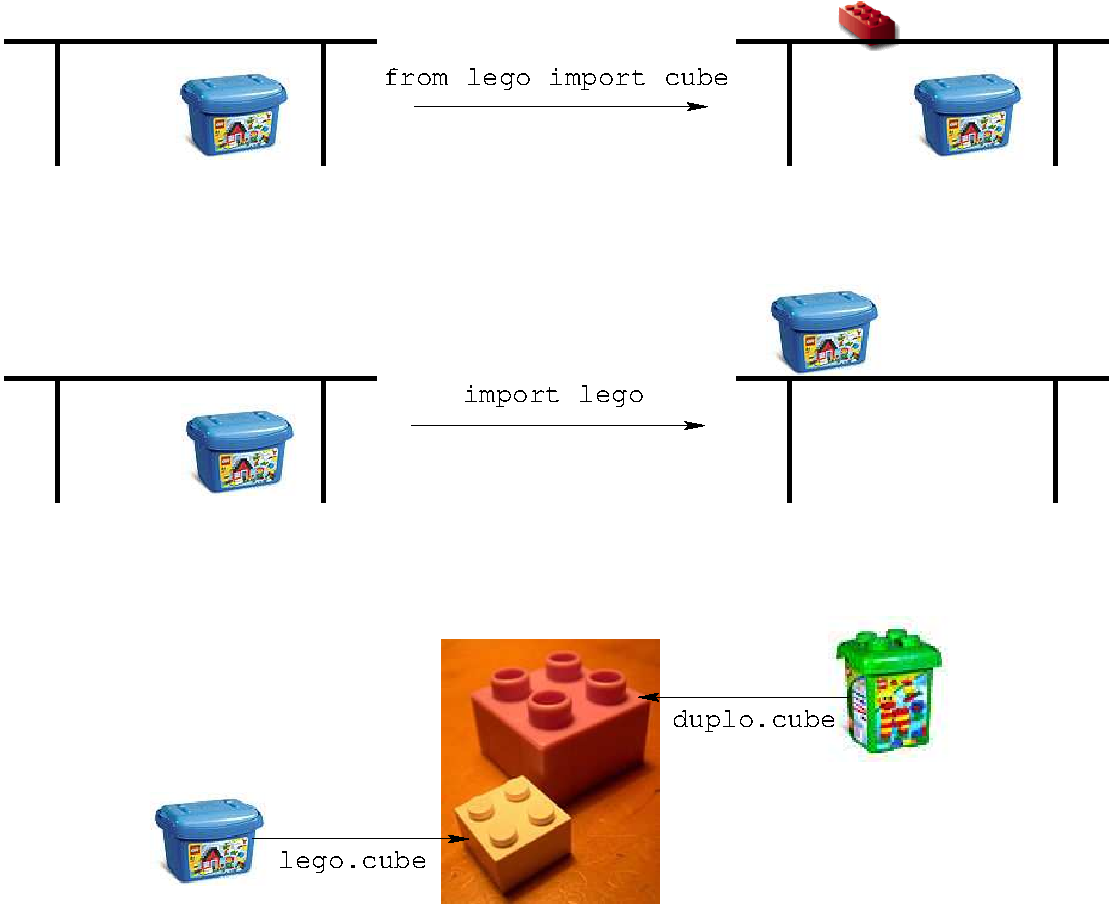
\includegraphics[width=7cm]{lego.pdf}$$
\end{fig}

\begin{rem}
{\sc Lego} est une société danoise fabriquant des jeux dont le produit phare
est un jeu de briques en plastique à assembler.
\end{rem}}
Ainsi en {\sc Python}, il existe de nombreux modules additionnels dont le plus 
connu est le module {\tt math} qui définit une vingtaine de constantes et fonctions mathématiques
usuelles (figure~\ref{fig:python:math}).
On peut importer ce module de différentes manières :

\noindent\mbox{}\hfill
\begin{py}{5cm}

\begin{verbatim}
>>> from math import sin, pi
>>> sin(pi/2)
1.0
\end{verbatim}
\end{py}
\hfill
\begin{py}{5cm}
\begin{verbatim}
>>> import math
>>> math.sin(math.pi/2)
1.0
\end{verbatim}
\end{py}
\hfill\mbox{}
\vspace*{1mm}

\noindent Pour comprendre la différence entre ces deux méthodes, aidons-nous de la métaphore 
des cubes {\em à la {\sc Lego}} (figure \ref{fig:lego}). Nous disposons d'une boîte de cubes 
({\tt lego}) rangée sous la table. 
Pour utiliser un cube de cette boîte, nous pouvons soit prendre le cube 
dans la boîte et le mettre sur la table ({\tt from lego import cube}) : le cube est alors 
directement accessible sur la table ({\tt cube}); soit mettre la boîte sur la table ({\tt import lego}) :
le cube n'est alors pas directement accessible, il faut encore le prendre dans la boîte 
({\tt lego.cube}). L'intérêt de cette deuxième méthode est de distinguer 2 cubes qui porteraient
le même nom ({\tt cube}) mais qui ne seraient pas originaires de la même boîte 
(boîtes {\tt lego} et {\tt duplo}) et qui seraient donc différents 
({\tt lego.cube} et {\tt duplo.cube}). Il est possible également de verser tout le contenu 
de la boîte sur la table ({\tt from lego import *}) : ici, l'astérisque ({\tt *}) signifie « tout ».

\noindent\mbox{}\hfill
\begin{py}{5cm}
\begin{verbatim}
>>> from math import *
>>> sqrt(tan(log(pi)))
1.484345173593278
\end{verbatim}
\end{py}
\hfill\mbox{}

%-------------------------------------------------------------------------
\section{Définition d'une fonction}\label{definition}
%-------------------------------------------------------------------------
\noindent Pour encapsuler un algorithme dans une fonction, on suivra pas à pas 
la démarche suivante :
\begin{enumerate}
\item donner un nom explicite à l'algorithme,
\item définir les paramètres d'entrée-sortie de l'algorithme,
\item préciser les préconditions sur les paramètres d'entrée,
\item donner des exemples d'utilisation et les résultats attendus,
\item décrire par une phrase ce que fait l'algorithme et dans quelles conditions il le fait,
\item encapsuler l'algorithme dans la fonction spécifiée par les 5 points
	précédents.
\end{enumerate}
Les 5 premières étapes relèvent de la spécification de l'algorithme et la
dernière étape concerne l'encapsulation proprement dite de l'algorithme.
En \python, la spécification sera exécutable : à chaque étape, le code de la fonction 
est toujours exécutable même s'il ne donne pas encore le bon résultat; seule la dernière 
étape d'encapsulation (voir section \ref{sub:encapsuler} page \pageref{sub:encapsuler})
permettra d'obtenir le résultat valide attendu.

\begin{defin}[spécification d'un algorithme]\index[def]{spécification d'un algorithme}\index{fonction!spécification}
La spécification d'un algorithme décrit ce que fait l'algorithme 
et dans quelles conditions il le fait.
\end{defin}

\begin{defin}[implémentation d'un algorithme]\index[def]{implémentation d'un algorithme}\index{fonction!implémentation}
L'implémentation d'un algorithme décrit comment fait l'algorithme 
pour satisfaire sa spécification.
\end{defin}

\begin{ex}[Nombres de Fibonacci]\label{ex:fibonacci}\index[algo]{nombres de {{\sc Fibonacci}}|(}
La fonction de Fibonacci calcule le nombre $u_n$ à l'ordre $n$ (dit de Fibonacci) 
selon la relation de récurrence :
$$u_0 = 1\ ,\ u_1 = 1\ ,\ u_n = u_{n-1} + u_{n-2}\ \forall n \in N,\ n > 1$$
Les 10 premiers nombres de Fibonacci valent donc : $u_0 = 1$, $u_1 = 1$, $u_2 = 2$,
$u_3 = 3$, $u_4 = 5$, $u_5 = 8$, $u_6 = 13$, $u_7 = 21$, $u_8 = 34$ et $u_9 = 55$.
\end{ex}
\noindent Dans cette section, nous utiliserons cet exemple comme fil conducteur
dans la définition d'une fonction. Ainsi donc, nous voulons définir une fonction
qui calcule le $n^{i\grave eme}$ nombre de Fibonacci. Cette description de la fonction
(« calculer le $n^{i\grave eme}$ nombre de Fibonacci ») évoluera progressivement
à chaque étape et deviendra suffisamment précise pour qu'un autre utilisateur puisse
l'utiliser effectivement sans surprise et en toute sécurité.


%-------------------------------------------------------------------------
\subsection{Nommer}\label{sub:nommer}
%-------------------------------------------------------------------------
La première chose à faire est de nommer la fonction qui encapsule l'algorithme. 
Les noms de fonction sont des identificateurs arbitraires, de préférence 
assez courts mais aussi explicites que possible, de manière à exprimer 
clairement ce que la fonction est censée faire. 
Les noms des fonctions doivent en outre obéir à quelques règles simples :
\begin{itemize}
\item Un nom de fonction est une séquence de lettres (a\ldots  z , A\ldots  Z) 
	et de chiffres (0\ldots  9), qui
      	doit toujours commencer par une lettre.
\item Seules les lettres ordinaires sont autorisées. Les lettres accentuées, 
	les cédilles, les espaces, les
      	caractères spéciaux tels que {\tt \$}, {\tt \#}, {\tt @}, etc. sont interdits, 
      	à l'exception du caractère {\tt \_} (souligné).
\item La « casse » est significative : les caractères majuscules et minuscules 
	sont distingués. Ainsi,
      	{\tt sinus}, {\tt Sinus}, {\tt SINUS} sont des fonctions différentes. 
\item Par convention, on écrira l'essentiel des noms de fonction en caractères minuscules (y compris la
	première lettre). On n'utilisera les majuscules qu'à l'intérieur même du nom  
	pour en augmenter éventuellement la lisibilité, comme dans {\tt triRapide} ou
	{\tt triFusion}.
\marginpar{\em\footnotesize
\begin{fig}[Mots réservés en {\sc Python}]\label{fig:motscles}\tt
$$\begin{tabular}{lllll}
        and       & del       & for       & is        & raise \\
        assert    & elif      & from      & lambda    & return\\
        break     & else      & global    & not       & try\\
        class     & except    & if        & or        & while\\
        continue  & exec      & import    & pass      & with\\
        def       & finally   & in        & print     & yield
\end{tabular}$$
\end{fig}}
\item Le langage lui-même peut se réserver quelques noms comme c'est le cas pour {\sc Python} 
	(figure \ref{fig:motscles}). Ces mots réservés ne peuvent donc pas être
	utilisés comme noms de fonction.
\end{itemize}
En ce qui concerne la fonction de Fibonacci de l'exemple \ref{ex:fibonacci}, 
nous choisissons de l'appeler simplement {\tt fibonacci}. Ce qui se traduira en {\sc Python} par
l'en-tête suivante où {\tt def} et {\tt return} sont deux mots réservés par {\sc Python}
pour définir les fonctions (voir annexe \ref{python:def} page \pageref{python:def}) :

\noindent\mbox{}\hspace*{1cm}\begin{py}{6cm}
\begin{verbatim}
def fibonacci():
    return
\end{verbatim}
\end{py}\hfill
\begin{py}{6cm}
\begin{verbatim}
>>> from fibo import fibonacci
>>> fibonacci()
>>>
\end{verbatim}
\end{py}
\hspace*{1cm}\mbox{}\vspace*{2mm}

\noindent Le code de la partie gauche est la définition actuelle de la fonction
{\tt fibonacci} que l'on a éditée dans un fichier {\tt fibo.py} :
le module associé a donc pour nom {\tt fibo}. 
La partie droite montre comment on utilise couramment le module {\tt fibo}
et la fonction {\tt fibonacci} sous l'interpréteur {\sc Python}.
Dans l'état actuel, cette fonction n'a pas d'arguments et ne fait rien ! 
Mais elle est déjà compilable et exécutable.
On peut la décrire de la manière suivante :
« La fonction {\tt fibonacci} calcule un nombre de Fibonacci ».

%-------------------------------------------------------------------------
\subsection{Paramétrer}\label{sub:parametrer}
%-------------------------------------------------------------------------
Un algorithme est une suite ordonnée d'instructions qui indique la démarche 
à suivre pour résoudre une série de problèmes équivalents. Dans ce contexte, 
c'est le paramétrage de l'algorithme qui lui donnera cette capacité recherchée
de résoudre des problèmes équivalents. Dans l'exemple de la fonction
{\tt sin}, c'est en effet le paramètre {\tt x} qui permet de calculer
le sinus de n'importe quel nombre réel ({\tt sin(x)}) et non le sinus d'un
seul nombre.
\marginpar{\em\footnotesize
\begin{fig}[Paramètres d'une fonction]\label{fig:fonction}
$$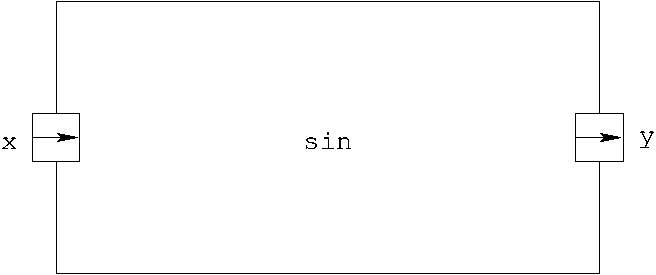
\includegraphics[width=5cm]{fonction1-1.pdf}$$
{\tt sin} est le nom de la fonction;
{\tt x} est le seul paramètre d'entrée,
{\tt y} le seul paramètre de sortie.
$$\mbox{\tt y = sin(x)}$$
$$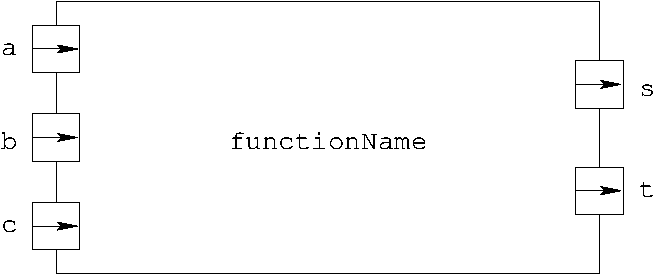
\includegraphics[width=5cm]{fonction3-2.pdf}$$
{\tt functionName} est le nom de la fonction;
{\tt a}, {\tt b} et {\tt c} sont les 3 paramètres d'entrée,
{\tt s} et {\tt t} les 2 paramètres de sortie.
$$\mbox{\tt (s,t) = functionName(a,b,c)}$$
\end{fig}}
La deuxième étape de la définition d'une fonction consiste donc
à préciser les paramètres d'entrée-sortie de la fonction (figure \ref{fig:fonction}).

\begin{defin}[paramètre d'entrée]\index[def]{paramètre d'entrée}\index{fonction!paramètre d'entrée}
Les paramètres d'entrée d'une fonction sont les arguments de la fonction
qui sont nécessaires pour effectuer le traitement associé à la fonction.
\end{defin}

\begin{defin}[paramètre de sortie]\index[def]{paramètre de sortie}\index{fonction!paramètre de sortie}
Les paramètres de sortie d'une fonction sont les résultats retournés 
par la fonction après avoir effectué le traitement associé à la fonction.
\end{defin}

Pour cela, on nomme ces paramètres avec des identificateurs
explicites dans le contexte courant d'utilisation de la fonction.
Les paramètres de sortie seront systématiquement initialisés à une valeur par défaut
(par exemple : {\tt 0} pour un entier, {\tt False} pour un booléen,
{\tt 0.0} pour un réel, {\tt ''} pour une chaîne de caractères,
{\tt []} pour un tableau).

La fonction {\tt fibonacci} prend l'ordre {\tt n} en paramètre d'entrée et
retourne le nombre {\tt u} ($u_n$). Le paramètre de sortie {\tt u} est un entier 
qui sera donc {\em a priori} initialisé à {\tt 0} dans la fonction
et qui sera retourné par la fonction ({\tt return u}).

\noindent\mbox{}\hspace*{1cm}\begin{py}{6cm}
\begin{verbatim}
def fibonacci(n):
    u = 0
    return u
\end{verbatim}
\end{py}\hfill
\begin{py}{6cm}
\begin{verbatim}
>>> from fibo import fibonacci
>>> fibonacci(5)
0
>>> fibonacci(-5)
0
>>> fibonacci('n')
0
\end{verbatim}
\end{py}
\hspace*{1cm}\mbox{}\vspace*{2mm}

\noindent  Le code de la partie gauche est la nouvelle définition de la fonction
{\tt fibonacci} toujours éditée dans le même fichier {\tt fibo.py} que précédemment. 
La partie droite montre son utilisation sous l'interpréteur {\sc Python}.
\marginpar{\em\footnotesize\vspace*{-5mm}
\begin{fig}[Fonction {\tt fibonacci} (1)]\label{fig:fibo1}
$$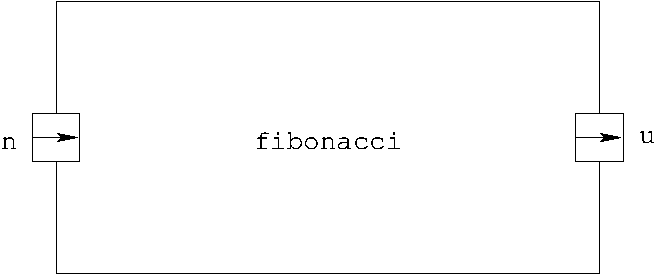
\includegraphics[width=5cm]{fibo-1.pdf}$$
{\tt fibonacci} est le nom de la fonction;
{\tt n} est le seul paramètre d'entrée,
{\tt u} le seul paramètre de sortie.
$$\mbox{\tt u = fibonacci(n)}$$
\end{fig}
\begin{fig}[Robustesse d'un algorithme]\label{fig:robustesse}
La robustesse d'un algorithme est son aptitude à se protéger de conditions 
anormales d'utilisation.
\end{fig}
\begin{fig}[L'instruction {\tt assert} en \python]\label{fig:python:assert}
{\tt assert expr[, message]} 	 
\vspace*{2mm}

{\tt expr} est évaluée : 
si {\tt expr == True}, on passe à l'instruction suivante,
sinon l'exécution est interrompue et 
une exception {\tt AssertionError} est levée qui affiche le {\tt message} optionnel.
%\vspace*{3mm}

Exemple :\\
\mbox{}\hfill\begin{py}{7cm}\tt
>>> assert False, "message d'erreur"\\
Traceback (most recent call last):\\
\mbox{}\ \ File "<stdin>", line 1, in <module>\\
AssertionError: message d'erreur\\
>>>
\end{py}
\end{fig}
}
Dans l'état actuel, cette fonction retourne {\tt 0} quels que soient le type et la valeur
du paramètre d'entrée ! 
Mais elle est encore compilable et exécutable.
On peut maintenant la décrire de la manière suivante :
« {\tt u = fibonacci(n)} est le $n^{i\grave eme}$ nombre de Fibonacci » (figure~\ref{fig:fibo1}).
Cette description est un peu moins « littéraire » que dans la section \ref{sub:nommer} précédente.
Elle a cependant l'avantage de montrer l'utilisation typique de la fonction
({\tt u = fibonacci(n)}) et d'expliciter le sens des paramètres d'entrée-sortie
({\tt n} et {\tt u}).

%-------------------------------------------------------------------------
\subsection{Protéger}
%-------------------------------------------------------------------------
Dans la section précédente, nous avons testé la fonction {\tt fibonacci}
avec comme paramètre d'entrée la chaîne de caractères {\tt 'n'} : 
cela n'a aucun sens pour le calcul d'un nombre de Fibonacci ! Il faut
donc protéger la fonction pour la rendre plus robuste face à des contextes
anormaux d'utilisation (figure \ref{fig:robustesse}). 
Pour cela, on imposera
aux paramètres d'entrée de vérifier certaines conditions avant
d'exécuter la fonction appelée. Ces conditions préalables à l'exécution
sont appelées les préconditions.

\begin{defin}[précondition]\index[def]{précondition}\index{fonction!précondition}
Les préconditions d'une fonction sont les conditions que doivent 
impérativement vérifier les paramètres d'entrée de la fonction
juste avant son exécution.
\end{defin}

Une précondition est donc une expression booléenne qui prend soit la valeur 
{\tt False} (faux) soit la valeur {\tt True} (vrai). 
Elle peut contenir des opérateurs de comparaison ({\tt ==}, {\tt !=}, {\tt >}, {\tt >=}, {\tt <=}, {\tt <}),
des opérateurs logiques ({\tt not}, {\tt and}, {\tt or}), des opérateurs d'identité ({\tt is},
{\tt is not}), des opérateurs d'appartenance ({\tt in}, {\tt not in}) ou toutes autres fonctions booléennes.
En \python, on définira les préconditions que doivent vérifier les paramètres
d'entrée de la fonction à l'aide de la directive {\tt assert} (figure \ref{fig:python:assert}). 
A l'exécution du code, cette directive « lèvera une exception~»
si la condition (l'assertion, figure \ref{fig:dico8}) testée est fausse.
Les préconditions seront placées systématiquement juste après l'en-tête
de la fonction ({\tt def fibonacci(n):}).

\noindent\mbox{}\hspace*{1cm}\begin{py}{6cm}
\begin{verbatim}
def fibonacci(n):
    assert type(n) is int
    assert n >= 0
    u = 0
    return u
\end{verbatim}
\end{py}\hfill
\begin{py}{6cm}
\begin{verbatim}
>>> fibonacci(-5)
Traceback ...
    assert n >= 0
AssertionError
>>> fibonacci('n')
Traceback ...
    assert type(n) is int
AssertionError
\end{verbatim}
\end{py}
\hspace*{1cm}\mbox{}\vspace*{2mm}

\marginpar{\em\footnotesize
\begin{fig}[Définition de l'Académie (8)]\label{fig:dico8}
\mbox{}\\
{\em ASSERTION} n. f. XIIIe siècle. Emprunté du latin assertio, dérivé de assertum, 
supin de asserere, « revendiquer », puis « prétendre, affirmer ».
Proposition qu'on avance et qu'on soutient comme vraie. 
\end{fig}
\begin{fig}[Fonction {\tt fibonacci} (2)]\label{fig:fibo2}
$$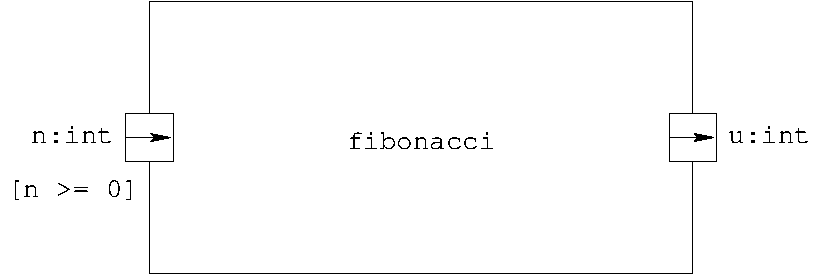
\includegraphics[width=5cm]{fibo-2.pdf}$$
{\tt n:int} est le paramètre d'entrée de nom {\tt n} et de type {\tt int}
qui doit vérifier la précondition {\tt [n >= 0]}.\\
{\tt u:int} est la paramètre de sortie de nom {\tt u} et de type {\tt int}.
$$\mbox{\tt u = fibonacci(n)}$$
\end{fig}}
\noindent La définition de la fonction {\tt fibonacci} a donc été complétée par les préconditions
sur le paramètre d'entrée : $n$ doit être un entier ({\tt type(n) is int})
positif ou nul ({\tt n >= 0}). 
Sa description peut alors être complétée pour tenir compte de ces préconditions 
sur l'ordre {\tt n} du nombre de Fibonacci calculé :
«~{\tt u = fibonacci(n)} est le $n^{i\grave eme}$ nombre de Fibonacci si
{\tt n:int >= 0}~» (figure \ref{fig:fibo2}).
La fonction est toujours compilable et exécutable, mais son
exécution est maintenant systématiquement interrompue si les préconditions ne sont pas 
respectées : ce qui est le cas pour les paramètres d'entrée {\tt -5} et {\tt 'n'}.
Dans tous les autres cas (entiers positifs ou nuls), elle retourne toujours {\tt 0} !

En \python, la manière dont nous avons initialisé le paramètre de sortie {\tt u}
({\tt u = 0}) indique qu'il s'agit implicitement d'un entier ({\tt int}). La fonction
{\tt fibonacci} retourne donc un entier : c'est une postcondition 
sur le paramètre de sortie {\tt u} dans le cas du calcul d'un nombre de Fibonacci.

\begin{defin}[postcondition]\index[def]{postcondition}\index{fonction!postcondition}
Les postconditions d'une fonction sont les conditions que doivent 
impérativement vérifier les paramètres de sortie de la fonction
juste après son exécution.
\end{defin}

En plus des préconditions et des postconditions, on pourra quelquefois imposer
que des conditions soient vérifiées tout au long de l'exécution de la fonction :
on parle alors d'invariants. 

\begin{defin}[invariant de fonction]\index[def]{invariant}\index{fonction!invariant}
Les invariants d'une fonction sont les conditions que doit 
impérativement vérifier la fonction tout au long de son exécution.
\end{defin}

\noindent De tels exemples d'invariants seront mis en évidence 
lors de l'implémentation de certaines fonctions.


%-------------------------------------------------------------------------
\subsection{Tester}
%-------------------------------------------------------------------------
Avant même d'implémenter la fonction proprement dite (voir section 
\ref{sub:encapsuler}), on définit des tests que devra vérifier la 
fonction une fois implémentée. Ces tests sont appelés tests unitaires
car ils ne concernent qu'une seule fonction, la fonction que l'on cherche
à définir.
Ce jeu de tests constitue ainsi un ensemble caractéristique d'entrées-sorties associées
que devra vérifier la fonction. 
Par exemple,
{\tt fibonacci(0)} devra retourner {\tt 1}, {\tt fibonacci(1)} devra retourner {\tt 1}, 
{\tt fibonacci(2)} devra retourner {\tt 2} ou encore {\tt fibonacci(9)} devra retourner {\tt 55}.
En fait, quelle que soit la manière dont sera implémentée la fonction {\tt fibonacci},
les résultats précédents devront être obtenus par cette implémentation.

En \python, on utilisera une {\tt docstring} (chaîne entre 3 guillemets : {\tt """ \ldots\ """}) pour
décrire ces tests.
Cette chaîne spéciale, placée entre l'en-tête et les préconditions et qui peut tenir
sur plusieurs lignes, joue le rôle de commentaire dans le corps de la fonction.
Elle ne change donc {\em a priori} rien à son exécution courante. 

\noindent\mbox{}\hspace*{1cm}\begin{py}{6cm}
\begin{verbatim}
def fibonacci(n):
    """
    >>> fibonacci(0)
    1
    >>> fibonacci(2)
    2
    >>> fibonacci(9)
    55
    """
    assert type(n) is int
    assert n >= 0
    u = 0
    return u
\end{verbatim}
\end{py}\hfill
\begin{py}{6cm}
\begin{verbatim}
>>> fibonacci(0)
0
>>> fibonacci(2)
0
>>> fibonacci(9)
0
\end{verbatim}
\end{py}
\hspace*{1cm}\mbox{}\vspace*{2mm}

\noindent Nous avons donc ajouter 3 tests dans la définition de la fonction {\tt fibonacci}.
En \python, ces tests ont la particularité de se présentent sous la même forme
que lorsqu'on appelle la fonction sous l'interpréteur \python, à ceci près qu'ils sont
écrits dans une {\tt docstring} ({\tt """ \ldots\ """}) :\\
\noindent\mbox{}\hspace*{1cm}\begin{py}{6cm}
\begin{verbatim}
"""
>>> fibonacci(0)
1
>>> fibonacci(2)
2
>>> fibonacci(9)
55
"""
\end{verbatim}
\end{py}
\hfill
\begin{py}{6cm}
\begin{verbatim}
>>> fibonacci(0)
0
>>> fibonacci(2)
0
>>> fibonacci(9)
0
\end{verbatim}
\end{py}
\hspace*{1cm}\mbox{}\vspace*{2mm}

\marginpar{\footnotesize\em
\begin{fig}[Le module {\tt doctest}]\label{fig:doctest}
Le module {\tt doctest} est un module standard \python\ 
qui offre des services pour manipuler les {\tt docstring}s 
utilisées dans les jeux de tests :\\
\href{http://www.python.org/doc/2.5/lib/module-doctest.html}{\tt www.python.org/doc/2.5/lib/module-doctest.html}\\
\mbox{}

The doctest module searches for pieces of text that look like 
interactive \python\ sessions, and then executes those sessions 
to verify that they work exactly as shown. 
There are several common ways to use doctest:
\begin{itemize}
\item To check that a module's docstrings are up-to-date by verifying 
      that all interactive examples still work as documented.
\item To perform regression testing by verifying that interactive examples 
      from a test file or a test object work as expected.
\item To write tutorial documentation for a package, liberally illustrated 
      with input-output examples. Depending on whether the examples or 
      the expository text are emphasized, this has the flavor of "literate testing" 
      or "executable documentation".
\end{itemize}
The functions {\tt testmod()} and {\tt testfile()} provide a simple interface 
to {\tt doctest} that should be sufficient for most basic uses. 
\end{fig}}
\noindent La fonction est toujours compilable et exécutable, et son exécution retourne toujours {\tt 0}.
Si maintenant, nous ajoutons les 3 lignes ci-dessous à la fin du fichier {\tt fibo.py},
les tests que nous avons ajoutés à la définition de la fonction {\tt fibonacci} vont
être évalués automatiquement (figure~\ref{fig:doctest}) comme le montre l'exécution de la page suivante.

\noindent\mbox{}\hspace*{1cm}\begin{py}{6cm}
\begin{verbatim}
if __name__ == "__main__" :
    import doctest
    doctest.testmod()
\end{verbatim}
\end{py}
\hspace*{1cm}\mbox{}\vspace*{2mm}

\noindent D'une certaine manière ces tests permettent de préciser ce qu'on attend de la fonction.
Le choix de ces tests est donc très important pour valider l'implémentation future.

\noindent\mbox{}\hspace*{1cm}\begin{py}{6cm}
\begin{verbatim}
$ python fibo.py
**********************************************
File "fibo.py", line 10, in __main__.fibonacci
Failed example:
    fibonacci(0)
Expected:
    1
Got:
    0
**********************************************
File "fibo.py", line 12, in __main__.fibonacci
Failed example:
    fibonacci(2)
Expected:
    2
Got:
    0
**********************************************
File "fibo.py", line 14, in __main__.fibonacci
Failed example:
    fibonacci(9)
\end{verbatim}
\end{py}
\hfill
\begin{py}{6cm}
On lance l'interpréteur \python\ en passant le fichier à tester
(ici {\tt fibo.py}). Chaque test du jeu de tests placé dans
la {\tt docstring} de la fonction à tester sera exécuté par
l'interpréteur. Si le résultat du test est conforme à ce qui était prévu
(par exemple {\tt factorielle(0)} $\rightarrow$ {\tt 1}), rien de particulier
ne se passe. Si le test est en erreur, \python\ précise
la ligne du fichier où apparaît le test
(par exemple : {\tt File "fibo.py", line 10}), le test en
erreur ({\tt fibonacci(0)}), le résultat attendu
({\tt Expected: 1}) et le résultat obtenu ({\tt Got: 0}).
Ainsi, on peut vérifier simplement si la fonction
a passé le jeu de tests. C'est une manière de tester la validité 
de l'implémentation.
\end{py}

\noindent\mbox{}\hspace*{1cm}\begin{py}{6cm}
\begin{verbatim}
Expected:
    55    
Got:
    0
**********************************************
1 items had failures:
   3 of   3 in __main__.fibonacci
***Test Failed*** 3 failures.
$
\end{verbatim}
\end{py}
\hspace*{1cm}\mbox{}\vspace*{2mm}

\noindent Ces tests seront conservés tant que la fonctionnalité est requise. 
A chaque modification du code, on effectuera tous les tests ainsi définis 
pour vérifier si quelque chose ne fonctionne plus.

%-------------------------------------------------------------------------
\subsection{Décrire}
%-------------------------------------------------------------------------
Une fois choisis le nom de la fonction, les paramètres d'entrée-sortie, les préconditions
sur les paramètres d'entrée et les jeux de tests, on peut alors préciser « ce que fait l'algorithme » 
et «~dans quelles conditions il le fait » :
il s'agit d'une phrase de description « en bon français~» qui permettra
à tout utilisateur de comprendre ce que fait l'algorithme sans 
nécessairement savoir comment il le fait.

\begin{defin}[description d'une fonction]\index[def]{description d'une fonction}\index{fonction!description}
La description d'une fonction est une phrase qui précise ce que fait la fonction 
et dans quelles conditions elle le fait.
\end{defin}

Cette phrase est une chaîne de caractères qui doit expliciter le rôle
des paramètres d'entrée et leurs préconditions, ainsi que toutes autres informations
jugées nécessaires par le concepteur de la fonction. 
En particulier, lorsque le retour de la fonction n'est pas « évident », on 
explicitera les paramètres de sortie. Dans le cas de la fonction {\tt fibonacci},
un utilisateur de la fonction «~saura~» ce qu'est un nombre de Fibonacci et la précision
que cette fonction retourne un entier n'est pas nécessaire. Par contre, si la fonction 
retourne plus d'une valeur, il faut au moins préciser l'ordre dans lequel elle les retourne.
Ainsi par exemple, pour la fonction {\tt divmod(a,b)} de la bibliothèque standard 
\python\ qui calcule le quotient {\tt q} et le reste {\tt r} de la division entière $a\div b$
(voir annexe \ref{python:fonctions} page \pageref{python:fonctions}), il faut préciser
qu'elle retourne un n-uplet ({\em tuple}) dans l'ordre {\tt (q,r)}. 
Dans certains cas, il faut
également préciser que la fonction effectue les calculs dans telles ou telles unités : c'est 
par exemple le cas des fonctions trigonométriques usuelles où les calculs sont menés avec 
des angles en radians (figure \ref{fig:python:math} page \pageref{fig:python:math}). 
Dans d'autres cas encore, on pourra préciser une référence bibliographique ou un site {\sc Web}
où l'utilisateur pourra trouver des compléments sur la fonction et l'algorithme associé.
La description d'une fonction intègrera donc au moins :
\begin{itemize}
\item un exemple typique d'appel de la fonction,
\item la signification des paramètres d'entrée-sortie,
\item les préconditions sur les paramètres d'entrée,
\item un jeu de tests significatifs.
\end{itemize}
Ainsi, la description de la fonction {\tt fibonacci} pourra se présenter sous la forme suivante :\\
« {\tt u = fibonacci(n)} est le nombre de Fibonacci à l'ordre {\tt n} si {\tt n:int >= 0}.\\
Exemples : {\tt fibonacci(0) $\rightarrow$ 1}, {\tt fibonacci(2) $\rightarrow$ 2}, 
{\tt fibonacci(9) $\rightarrow$ 55} ».

En {\sc Python}, on intègrera cette description dans la {\tt docstring} (chaîne entre 3 guillemets) 
que l'on a déjà utilisée pour le jeu de tests. Les exemples seront donnés sous la forme d'un jeu de tests
{\em à la \python}.
Cette chaîne spéciale, qui peut tenir
sur plusieurs lignes, joue le rôle de commentaire dans le corps de la fonction.
Elle ne change donc rien à son exécution. Par contre, 
elle permettra de documenter automatiquement l'aide en-ligne de \python\ ({\tt help})
ou encore, elle pourra être utilisée par certains environnements ({\tt idle} par exemple) 
ou par certains utilitaires comme {\tt pydoc} 
(voir annexe \ref{python:pydoc} page \pageref{python:pydoc}).

\noindent\mbox{}\hspace*{1cm}\begin{py}{6cm}
\begin{verbatim}
def fibonacci(n):
    """ 
    u = fibonacci(n) 
    est le nombre de Fibonacci 
    à l'ordre n si n:int >= 0 
    >>> fibonacci(0)
    1
    >>> fibonacci(2)
    2
    >>> fibonacci(9)
    55
    """
    assert type(n) is int
    assert n >= 0
    u = 0
    return u
\end{verbatim}
\end{py}\hfill
\begin{py}{6cm}
\begin{verbatim}
>>> fibonacci(5)
0
>>> fibonacci(100)
0
>>> help(fibo.fibonacci)
Help on function fibonacci in module fibo:

fibonacci(n)
    u = fibonacci(n) 
    est le nombre de Fibonacci 
    à l'ordre n si n:int >= 0 
    >>> fibonacci(0)
    1
    >>> fibonacci(2)
    2
    >>> fibonacci(9)
    55
\end{verbatim}
\end{py}
\hspace*{1cm}\mbox{}\vspace*{2mm}

\noindent La fonction est toujours compilable et exécutable; elle est maintenant
documentable ({\tt help(fibo. fibonacci)}), mais retourne toujours {\tt 0} ! 
Il reste à l'implémenter.
\exo{td:decoder}

\marginpar{\footnotesize\em\vspace*{-4cm}
\begin{td}[Décodage base b $\rightarrow$ décimal]\label{td:decoder}\index[td]{décodage base b $\rightarrow$ décimal}
En section \ref{sub:reutiliser}, la valeur décimale d'un nombre entier
codé en base $b$ était obtenu par l'algorithme suivant :\\
{\tt \mbox{}\ \ \ \ }\begin{py}{7.5cm}\tt
>>> n = 0\\
>>> for i in range(len(code)):\\
... \mbox{}\ \ \ \ n = n + code[i]*b**(len(code)-1-i)\\
... \\
>>> 
\end{py}\\[1mm]
Spécifier une fonction qui encapsulera cet algorithme.
\end{td}

\begin{fig}[Fonction {\tt fibonacci} (3)]\label{fig:fibo3}
{\bf Spécification :}\\
\centerline{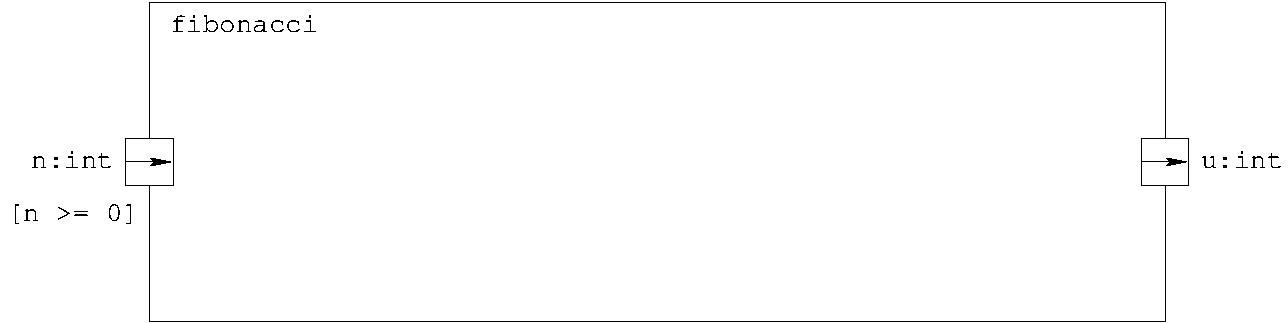
\includegraphics[width=7cm]{fibo-3.pdf}}
$$\begin{minipage}{6.5cm}
{\tt u = fibonacci(n)} est le nombre de Fibonacci à l'ordre {\tt n} si {\tt n:int >= 0}.\\
Exemples : 
\begin{minipage}[t]{3cm}
{\tt fibonacci(0) $\rightarrow$ 1}\\{\tt fibonacci(2) $\rightarrow$ 2}\\{\tt fibonacci(9) $\rightarrow$ 55}
\end{minipage}
\end{minipage}$$

{\bf Implémentation :}\\
\centerline{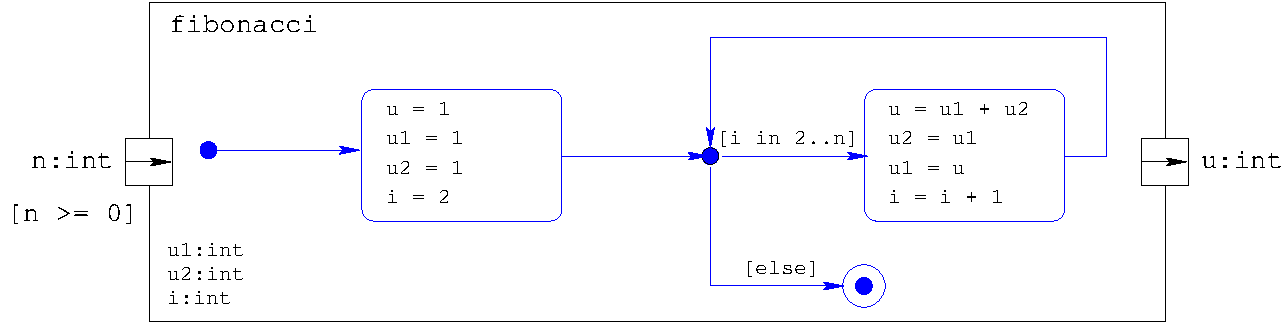
\includegraphics[width=7cm]{fibo-4.pdf}}
\end{fig}
}

%-------------------------------------------------------------------------
\subsection{Encapsuler}\label{sub:encapsuler}
%-------------------------------------------------------------------------
La dernière étape consiste enfin à dire « comment fait la fonction »
pour répondre à la spécification décrite au cours des étapes précédentes.
En phase de spécification, la fonction (ou la procédure) est vue comme 
une boîte noire dont on ne connaît pas le fonctionnement interne
(figure \ref{fig:fibo3} : spécification).
En phase d'implémentation, l'enchaînement des instructions nécessaires
à la résolution du problème considéré est détaillé (figure \ref{fig:fibo3} : implémentation).

\noindent\mbox{}\hspace*{1cm}\begin{py}{6cm}
\begin{verbatim}
>>> n
9
>>> u, u1, u2 = 1, 1, 1
>>> for i in range(2,n+1):
...     u = u1 + u2
...     u2 = u1
...     u1 = u
...
>>> u
55
\end{verbatim}
\end{py}\hfill
\begin{py}{6cm}
Compte-tenu de la définition des nombres de Fibonacci (exemple \ref{ex:fibonacci}),
les instructions ci-contre permettent de calculer le nombre {\tt u} de Fibonacci
pour un ordre {\tt n} donné (ici {\tt 9}). 
Pour chaque valeur de {\tt i}, {\tt u1} représente initialement le nombre de Fibonacci
à l'ordre {\tt (i-1)}, {\tt u2} le nombre de Fibonacci à l'ordre {\tt (i-2)} et {\tt u}
({\tt = u1 + u2}) le nombre de Fibonacci à l'ordre {\tt i}.
\end{py}
\hspace*{1cm}\mbox{}\vspace*{2mm}

Ce sont ces instructions qu'il faut 
encapsuler au c\oe ur de la fonction {\tt fibonacci} comme le montre le code complet ci-dessous
(voir remarque \ref{rem:fibonacci}).
\exo{td:codage}

\marginpar{\footnotesize\em
\begin{rem}\label{rem:fibonacci}
La suite de Fibonacci doit son nom au mathématicien italien Fibonacci (1175-1250). 
Dans un problème récréatif, Fibonacci décrit la croissance d'une population « idéale »
de lapins de la manière suivante :
\begin{itemize}
\item le premier mois, il y a juste une paire de lapereaux ;
\item les lapereaux ne sont pubères qu'à partir du deuxième mois ;
\item chaque mois, tout couple susceptible de procréer engendre effectivement 
	un nouveau couple de lapereaux ;
\item les lapins ne meurent jamais !
\end{itemize}
Se pose alors le problème suivant :
\begin{quote}\em
« Possédant initialement un couple de lapins, combien de couples obtient-on 
en douze mois si chaque couple engendre tous les mois un nouveau couple 
à compter du second mois de son existence ? »
\end{quote}
Ce problème est à l'origine de la suite de Fibonacci
dont le $n^{i\grave eme}$ terme correspond au nombre 
de couples de lapins au $n^{i\grave eme}$ mois. 
Au bout d'un an, il y aura donc {\tt fibonacci(12)} ($= 233$) couples de lapins 
dans cette population « idéale ». On n'ose à peine imaginer ce que serait cet univers 
« idéal » de lapins au bout de 10 ans ({\tt 8670007398507948658051921} couples !)\ldots
\end{rem}

\begin{td}[Codage des entiers positifs (2)]\label{td:codage}\index[td]{codage des entiers positifs}
Définir (spécifier et implémenter) une fonction qui 
code un entier $n$ en base $b$ sur $k$ chiffres
(voir TD \ref{td:codageEntier}).
\end{td}}
\noindent\mbox{}\hspace*{1cm}\begin{py}{6cm}
\begin{verbatim}
def fibonacci(n):
    """ 
    u = fibonacci(n) 
    est le nombre de Fibonacci 
    à l'ordre n si n:int >= 0 
    >>> fibonacci(0)
    1
    >>> fibonacci(2)
    2
    >>> fibonacci(9)
    55
    """
    assert type(n) is int
    assert n >= 0
    u, u1, u2 = 1, 1, 1
    for i in range(2,n+1):
        u = u1 + u2
        u2 = u1
        u1 = u
    return u
\end{verbatim}
\end{py}\hfill
\begin{py}{6cm}
\begin{verbatim}
>>> from fibo import fibonacci
>>> for n in range(10):
...     print(fibonacci(n),end=' ')
...
1 1 2 3 5 8 13 21 34 55
>>> for n in range(10,60,10):
...     print(fibonacci(n),end=' ')
...
89 10946 1346269 165580141 20365011074
>>> fibonacci(100)
573147844013817084101L
>>> fibo.fibonacci(120)
8670007398507948658051921L
>>> fibonacci(200)
453973694165307953197296969697410619233826L
\end{verbatim}
\end{py}
\index[algo]{nombres de {{\sc Fibonacci}}|)}
\mbox{}\hspace*{1cm}\vspace*{2mm}


\noindent En fait, plusieurs implémentations peuvent correspondre
à la même spécification. C'est le cas par exemple
pour le calcul de la somme des $n$ premiers nombres
entiers ci-dessous.

\index[algo]{suites numériques}
\noindent\mbox{}\hspace*{1cm}\begin{py}{6cm}
\begin{verbatim}
def sommeArithmetique(n):
    """
    s = sommeArithmetique(n) est la somme 
    des n premiers entiers si n:int >= 0
    >>> for n in range(7):
    ...     print(sommeArithmetique(n)\
                  == n*(n+1)/2,end=' ')
    True True True True True True True
    """
    assert type(n) is int
    assert n >= 0

    s = n*(n+1)/2
    
    return s
\end{verbatim}
\end{py}\hfill
\begin{py}{6cm}
\begin{verbatim}
def sommeArithmetique(n):
    """
    s = sommeArithmetique(n) est la somme 
    des n premiers entiers si n:int >= 0
    >>> for n in range(7):
    ...     print(sommeArithmetique(n)\
                  == n*(n+1)/2,end=' ')
    True True True True True True True
    """
    assert type(n) is int
    assert n >= 0

    s = 0
    for k  in range(1,n+1): s = s + k
    
    return s
\end{verbatim}
\end{py}
\hspace*{1cm}\mbox{}\vspace*{2mm}

L'implémentation de gauche repose directement sur le résultat
mathématique bien connu concernant les suites arithmétiques 
({\tt s = n*(n+1)/2} : voir remarque \ref{rem:suite}).
\marginpar{\footnotesize\em
\begin{rem}\label{rem:suite}La somme $S$ des $n$ premiers nombres entiers est telle que :
$$\displaystyle S = \sum_{k=1}^n k = (1 + 2 + 3 + \cdots + n) =
	\frac{n(n+1)}{2}$$
	\tiny En effet :
	$$\displaystyle\begin{array}[t]{rccccccccc}
	S &=& 1 &+& 2   &+& \cdots &+& n & \\
	S &=& n &+& n-1 &+& \cdots &+& 1 & \\
	\hline
	2S &=& (n+1) &+& (n+1) &+& \cdots &+& (n+1)\\
	\end{array}$$
	d'où : $\displaystyle 2S = n(n+1)$
\end{rem}

\begin{td}[Une spécification, des implémentations]\label{td:implem}\index[td]{spécification et implémentations}
\begin{enumerate}
\item Proposer deux implémentations du calcul de
la somme $s = \sum_0^n u_k$ des $n$ premiers termes d'une suite 
géométrique $u_k = a\cdot b^k$.
\item Comparer les complexités de ces deux im\-plé\-men\-ta\-tions.
\end{enumerate}
\end{td}}
L'implémentation de droite effectue la somme 1 à 1 des n premiers éléments ({\tt s = s + k}).
Ces deux implémentations sont toutes les deux conformes au jeu de tests, mais elles 
ne se valent pas en terme de complexité. La première est dite « à temps constant » : 
quelle que soit la valeur de $n$, le calcul ne nécessitera jamais plus de 3 opérations 
({\tt (n+1)}, {\tt n*(n+1)} et {\tt n*(n+1)/2}). La seconde est dite « à temps linéaire » :
le nombre d'opérations ({\tt s + k}) dépend linéairement de $n$ (il y a $(n-1)$ additions à calculer
pour $n>1$). La première implémentation est donc plus efficace que la deuxième et lui sera préférée.
\exo{td:implem}

Ce sera le rôle du concepteur d'un algorithme de définir 
sa spécification et d'en proposer une implémentation efficace.
L'utilisateur de la fonction, quant à lui, n'a pas à connaître
l'implémen\-ta\-tion; seule la spécification de la fonction le concerne
car elle lui est nécessaire pour appeler la fonction.

%-------------------------------------------------------------------------
\subsection{Conclure}
%-------------------------------------------------------------------------
L'algorithmique, ou science des algorithmes, s'intéresse à l'art de construire 
des algorithmes ainsi qu'à caractériser leur validité, leur robustesse
leur réutilisabilité, leur complexité ou encore leur efficacité. Certaines 
de ces caractéristiques générales (validité, robustesse, réutilisabilité) 
se concrètisent à la lumière des préconisations précédentes concernant 
la définition d'une fonction.

\begin{description}
\item[Validité :] La validité d'un algorithme est son aptitude à réaliser 
	exactement la tâche pour laquelle il a été conçu.
	
	{\em ie}: L'implémentation de la fonction doit être conforme aux jeux de tests.
\item[Robustesse :] La robustesse d'un algorithme est son aptitude à se 
	protéger de conditions anormales d'utilisation.

	{\em ie}: La fonction doit vérifier impérativement ses préconditions.
\item[Réutilisabilité :] La réutilisabilité d'un algorithme est son aptitude 
	à être réutilisé pour résoudre des tâches équivalentes à celle pour 
	laquelle il a été conçu.	

	{\em ie}: La fonction doit être correctement paramétrée.
\end{description}

\noindent Une fois la fonction définie (spécifiée et implémentée), 
il reste à l'utiliser (à l'appeler).


%-------------------------------------------------------------------------
\section{Appel d'une fonction}\label{appel}
%-------------------------------------------------------------------------
Une fonction s'utilise (s'« appelle ») sous la forme du nom de la fonction
suivi de parenthèses à l'intérieur desquelles on transmet (on « passe »)
zéro ou plusieurs arguments conformément à la spécification de la fonction.
Dans le cas de la fonction {\tt fibonacci}, on doit transmettre un argument
et un seul lors de l'appel de la fonction.

\noindent\mbox{}\hspace*{1cm}\begin{py}{6cm}
\begin{verbatim}
>>> fibonacci(9)
55
>>> fibonacci(5+4)
55
>>> fibonacci(8) + fibonacci(7)
55
\end{verbatim}
\end{py}\hfill
\begin{py}{6cm}
\begin{verbatim}
>>> y = fibonacci(9)
>>> y
55
>>> x = 9
>>> y = fibonacci(x)
>>> y
55
\end{verbatim}
\end{py}
\hspace*{1cm}\mbox{}\vspace*{2mm}

\noindent L'argument transmis peut tout aussi bien être une constante (par exemple {\tt 9}),
une variable (par exemple {\tt x}) ou toute expression dont la valeur est un entier positif ou
nul (par exemple {\tt 5+4}). Mais quel rapport existe-t-il entre ces arguments transmis
et les paramètres d'entrée-sortie de la fonction ({\tt n} et {\tt u} dans le cas de la fonction
{\tt fibonacci}) ? C'est le problème du « passage des paramètres » de l'instruction appelante
à la fonction appelée.

%-------------------------------------------------------------------------
\subsection{Passage des paramètres}\label{sub:passage}
%-------------------------------------------------------------------------
Dans la définition d'une fonction, la liste des paramètres d'entrée 
spécifie les informations à transmettre comme arguments lors de l'appel de la
fonction. Les arguments effectivement utilisés doivent être fournis dans le même 
ordre que celui des paramètres d'entrée correspondants : 
le premier argument sera affecté au premier paramètre d'entrée, 
le second argument sera affecté au second paramètre d'entrée, et ainsi de suite.

\noindent\mbox{}\hspace*{1cm}\begin{py}{6cm}
\bf Définition :
\begin{verbatim}
def fibonacci(n):
    ...
    return u
\end{verbatim}
\end{py}\hfill
\begin{py}{6cm}
\bf Appel :
\begin{verbatim}
>>> y = fibonacci(x)
\end{verbatim}
\end{py}
\hspace*{1cm}\mbox{}\vspace*{2mm}

Les paramètres introduits dans la définition sont appelés les paramètres formels
(par exemple {\tt n} dans la définition de la fonction {\tt fibonacci});
les paramètres passés en arguments sont appelés les paramètres effectifs
(par exemple {\tt x} dans l'appel {\tt fibonacci(x)}). 

\begin{defin}[paramètre formel]\index[def]{paramètre formel}\index{fonction!paramètre formel}
Un paramètre formel est un paramètre d'entrée d'une fonction
utilisé à l'in\-té\-rieur de la fonction appelée.
\end{defin}

\begin{defin}[paramètre effectif]\index[def]{paramètre effectif}\index{fonction!paramètre effectif}
Un paramètre effectif est un paramètre d'appel d'une fonction
utilisé à l'ex\-té\-rieur de la fonction appelée.
\end{defin}

\marginpar{\footnotesize\em
\begin{td}[Passage par valeur]\label{td:swap}\index[td]{passage par valeur}
On considère les codes suivants :

{\tt \mbox{}\ }\begin{py}{2.25cm}\tt
>>> x, y\\
(1, 2)\\
>>> tmp = x\\
>>> x = y\\
>>> y = tmp\\
>>> x, y\\
(2, 1)
\end{py}
\hfill
\begin{py}{3cm}\tt
def swap(x,y):\\
\mbox{}\ \ \ \ tmp = x\\
\mbox{}\ \ \ \ x = y\\
\mbox{}\ \ \ \ y = tmp\\
\mbox{}\ \ \ \ return
\end{py}
\hfill
\begin{py}{2.25cm}\tt
>>> x, y\\
(1, 2)\\
>>> swap(x,y)\\
>>> x, y\\
(1, 2)
\end{py}\\[1mm]
Expliquer la différence entre l'exécution de gauche et l'exécution de droite
en explicitant l'appel équivalent à l'appel {\tt swap(x,y)} dans l'exécution
de droite.
\end{td}}
Lors de l'appel d'une fonction, il y a copie des paramètres effectifs 
dans les paramètres formels : les valeurs des paramètres effectifs 
passés en argument sont affectées aux paramètres formels d'entrée 
correspondants (on parle de « passage par valeur » ou de « passage par copie »). 
Ainsi, ce ne sont pas les paramètres effectifs qui sont manipulés par la 
fonction elle-même mais des copies de ces paramètres. 
A la sortie de la fonction, on copie la valeur du paramètre 
formel de retour ({\tt u} dans la fonction {\tt fibonacci}) dans un paramètre 
effectif qui remplace temporairement l'appel de la fonction ({\tt fibonacci(x)})
et qui est finalement utilisé par l'instruction qui a appelé la fonction
(l'affectation dans le cas de l'instruction {\tt y = fibonacci(x)}).
Cette variable temporaire est ensuite détruite automatiquement.
Ainsi, l'instruction {\tt y = fibonacci(x)} est «~équivalente~» à la séquence 
d'instructions suivante (appel équivalent) :\index{fonction!appel équivalent}
\exo{td:swap}

\noindent\mbox{}\hspace*{1cm}\begin{py}{6cm}
{\bf Définition :}\\
{\tt
def fibonacci(n):\\
{\color{blue}
\mbox{}\ \ \ \ u, u1, u2 = 1, 1, 1\\
\mbox{}\ \ \ \ for i in range(2,n+1):\\
\mbox{}\ \ \ \ \ \ \ \ u = u1 + u2\\
\mbox{}\ \ \ \ \ \ \ \ u2 = u1\\
\mbox{}\ \ \ \ \ \ \ \ u1 = u}\\
\mbox{}\ \ \ \ return u\\
\mbox{}}
\end{py}\hfill
\begin{py}{6cm}
{\bf Appel :}\\\tt
%\begin{verbatim}
>>> x = 9\\
{\color{red}
>>> y = fibonacci(x)}\\
>>> y\\
55
\end{py}

\noindent\mbox{}\hspace*{1cm}\begin{py}{4.75cm}
{\bf Appel équivalent :}\\\tt
>>> x = 9\\
{\color{red} >>> n = x}\\
{\color{blue}
>>> u, u1, u2 = 1, 1, 1\\
>>> for i in range(2,n+1):\\
... \ \ \ \ u = u1 + u2\\
... \ \ \ \ u2 = u1\\
... \ \ \ \ u1 = u\\
...}\\
{\color{red} >>> tmp = u\\
>>> del n, u, u1, u2, i\\
>>> y = tmp\\
>>> del tmp}\\
>>> y\\
55
\end{py}
\hfill
\begin{py}{10cm}
\noindent On commence par copier la valeur du paramètre effectif {\tt x}
dans le paramètre formel d'entrée {\tt n} ({\color{red}\tt n = x});
en \python, {\tt n} est vraiment créée à ce moment là seulement.
On exécute ensuite «~tel quel~» le code de la fonction {\tt fibonacci} :
les variables internes à la fonction ({\tt u}, {\tt u1}, {\tt u2}, {\tt i})
sont créées et manipulées conformément à la définition de {\tt fibonacci}.
L'instruction «~{\tt return u}~» provoque ensuite la création d'une variable 
temporaire {\tt tmp} dans laquelle on copie la valeur du paramètre formel 
de sortie {\tt u} ({\color{red}\tt tmp = u}) et toutes les variables introduites
dans le corps de la fonction sont détruites
({\color{red}\tt del n, u, u1, u2, i}). On affecte la valeur de {\tt tmp} à {\tt y} ({\color{red}\tt y = tmp}) :
cette affectation réalise effectivement l'affectation souhaitée ({\tt y = fibonacci(x)}). 
Enfin, la variable temporaire {\tt tmp} introduite
au «~retour de la fonction~» {\tt fibonacci} est détruite ({\color{red}\tt del tmp}).
A la fin, seules coexistent les deux variables {\tt x} et {\tt y} : toutes les autres
variables ({\tt n}, {\tt u}, {\tt u1}, {\tt u2}, {\tt i} et {\tt tmp}) ont été
créées temporairement pour les besoins de l'appel de la fonction, puis détruites.
\end{py}
\hspace*{1cm}\mbox{}\vspace*{2mm}


\begin{defin}[passage par valeur]\index[def]{passage par valeur}\index{fonction!passage par valeur}
Le passage des paramètres par valeur (ou par copie) consiste à copier la valeur
du paramètre effectif dans le paramètre formel correspondant.
\end{defin}

Dans certains cas, le paramètre effectif occupe une trop grande place en mémoire 
pour envisager de le recopier. Par exemple, une image satellite de $6000\times 6000$
pixels codés sur 8 niveaux de gris occupe $36 Mo$ en mémoire; la copier conduirait
à occuper $72 Mo$ ! Par ailleurs, on peut vouloir effectuer un traitement
sur l'image originale et non traiter une de ses copies. Pour remedier à ces
problèmes liés au passage des paramètres par valeur, on utilisera 
le « passage par référence » qui consiste à transférer
la référence de la variable (son nom ou son adresse en mémoire) plutôt que sa valeur.

\begin{defin}[passage par référence]\index[def]{passage par référence}\index{fonction!passage par référence}
Le passage des paramètres par référence consiste à copier la référence
du paramètre effectif dans le paramètre formel correspondant.
\end{defin}

En \python, certains types de  variables utilisent systématiquement
le passage par référence : c'est le cas des listes (type {\tt list}), 
des dictionnaires (type {\tt dict}) ou encore
des classes (types définis par le programmeur).

\noindent\mbox{}\hspace*{1cm}\begin{py}{6cm}
\begin{verbatim}
def f(x):
    assert type(x) is list
    if len(x) > 0: x[0] = 5
    return

def g(x):
    assert type(x) is list
    y = [9,8,7]
    x = y
    x[0] = 5
    return
\end{verbatim}
\end{py}
\hfill
\begin{py}{6cm}
\begin{verbatim}
>>> t = [0,1,2]
>>> f(t)
>>> t
[5, 1, 2]

>>> t = [0,1,2]
>>> g(t)
>>> t
[0, 1, 2]
\end{verbatim}
\end{py}
\hspace*{1cm}\mbox{}\vspace*{2mm}

\marginpar{\footnotesize\em
\begin{rem}\label{rem:dico}Passage par référence pour les dictionnaires\\[1mm]
\begin{py}{4cm}\tt
def f(x):\\
\mbox{}\ \ \ \ assert type(x) is dict\\
\mbox{}\ \ \ \ x[0] = 5\\
\mbox{}\ \ \ \ return\\
\mbox{}\\
def g(x):\\
\mbox{}\ \ \ \ assert type(x) is dict\\
\mbox{}\ \ \ \ y = \{0\char`:9, 1\char`:8, 2\char`:7\}\\
\mbox{}\ \ \ \ x = y\\
\mbox{}\ \ \ \ x[0] = 5\\
\mbox{}\ \ \ \ return
\end{py}
\hfill
\begin{py}{3cm}\tt
>>> d = \{\}\\
>>> f(d)\\
>>> d\\
\{0: 5\}\\
\mbox{}\\
>>> d = \{\}\\
>>> g(d)\\
>>> d\\
\{\}
\end{py}
\end{rem}}\noindent Les fonctions {\tt f()} et {\tt g()} nécessitent chacune un argument 
de type {\tt list} ({\tt assert type(x) is list}).
Cet argument sera donc passé par référence lors de l'appel de ces fonctions :
à l'intérieur de chacune d'elles, on manipulera une copie de la référence de la liste 
passée en argument ({\tt t} dans les exemples de droite). 
La fonction {\tt f()} cherche à modifier
le premier élément de la liste ({\tt x[0] = 5}) : elle affecte au premier
élément de la liste nommée {\tt x} (l'élément de rang {\tt 0} : {\tt x[0]}) 
la valeur {\tt 5}. Comme le paramètre formel {\tt x} est une copie de la
référence originale {\tt t}, il référence le même tableau de valeurs {\tt [0,1,2]}
et la modification portera bien sur l'élément {\tt 0} du tableau original.
A la sortie de la fonction {\tt f()}, la liste {\tt t} originale est bien modifiée.
Quant à elle, la fonction {\tt g()} cherche à modifier la référence de la liste
{\tt x} ({\tt x = y}). En fait, elle modifie la copie de la référence ({\tt x})
mais pas la référence originale ({\tt t}). L'affectation suivante ({\tt x[0] = 5})
modifie ainsi le premier élément du tableau de valeurs {\tt [9,8,7]}.
Mais, à la sortie de la fonction {\tt g()},
le tableau de valeurs {\tt [0,1,2]} référencé par la liste {\tt t} originale 
n'est pas modifié.
Les mêmes fonctionnements sont obtenus avec un dictionnaire comme le montrent
les exemples de la remarque \ref{rem:dico} ci-contre.




%-------------------------------------------------------------------------
\subsection{Paramètres par défaut}
%-------------------------------------------------------------------------
Dans la définition d'une fonction, il est possible de définir une
valeur par défaut pour chacun des paramètres d'entrée. 
\index{fonction!paramètre par défaut}
On peut définir une valeur par défaut pour tous les paramètres, ou une partie d'entre eux
seulement; dans ce cas, les paramètres sans valeur par défaut doivent précéder les autres
dans la liste.
On obtient ainsi une fonction qui 
peut être appelée avec tous ses paramètres ou une partie seulement des arguments attendus :

\noindent\mbox{}\hspace*{1cm}\begin{py}{6cm}
\begin{verbatim}
def f(x, y = 0, z = 'r'):
    return x,y,z
\end{verbatim}
\end{py}
\hfill
\begin{py}{6cm}
\begin{verbatim}
>>> f(1,2,'t')
(1, 2, 't')
\end{verbatim}
\end{py}
\hspace*{1cm}\mbox{}\vspace*{2mm}

%\newpage
\noindent\mbox{}\hspace*{1cm}\begin{py}{6cm}
\begin{verbatim}
>>> f(1,2)
(1, 2, 'r')
>>> f(1)
(1, 0, 'r')
\end{verbatim}
\end{py}
\hfill
\begin{py}{6cm}
\begin{verbatim}
>>> f()
Traceback ...
TypeError: f() takes at least 1 argument
           (0 given)
\end{verbatim}
\end{py}
\hspace*{1cm}\mbox{}\vspace*{2mm}


\noindent De nombreuses fonctions des bibliothèques standards possèdent des
arguments par défaut. C'est le cas par exemple de la fonction standard {\tt int()} 
(voir annexe \ref{python:fonctions} page \pageref{python:fonctions})
ou encore de la fonction {\tt log()} du module {\tt math} 
(voir figure \ref{fig:python:math} page \pageref{fig:python:math}).

\noindent\mbox{}\hspace*{1cm}\begin{py}{6cm}
\begin{verbatim}
>>> int('45')
45
>>> int('45',10)
45
>>> int('101101',2)
45
>>> int('45',23)
97
>>> int('45',23) == 4*23**1 + 5*23**0
True
\end{verbatim}
\end{py}
\hfill
\begin{py}{6cm}
\begin{verbatim}
>>> from math import *
>>> e
2.7182818284590451
>>> log(e)
1.0
>>> log(e,e)
1.0
>>> log(e,10)
0.43429448190325176
>>> log(pi,7) == log(pi)/log(7)
True
\end{verbatim}
\end{py}
\hspace*{1cm}\mbox{}\vspace*{2mm}

\marginpar{\footnotesize\em
\begin{td}[Valeurs par défaut]\label{td:defaut}\index[td]{valeurs par défaut}
On considère la fonction qui code en base $b$ sur $k$ chiffres
un nombre décimal $n$ (voir TD \ref{td:codage}). 
Proposer une définition de cette fonction où $k = 8$ et $b = 2$ par défaut.
\end{td}}
\noindent A gauche, la fonction {\tt int()} permet de transformer en un entier décimal
une chaîne de caractères (par exemple {\tt '45'}) qui représente un nombre écrit dans la 
base spécifiée par le $2^{\grave eme}$ argument (par exemple {\tt 23}). Par défaut, cette
base est la base décimale ({\tt 10}). A droite, la fonction {\tt log()} calcule le logarithme
d'un nombre (par exemple {\tt 2.7182818284590451}) dans la base spécifiée par le 
$2^{\grave eme}$ argument (par exemple {\tt 10}). Par défaut, cette base est celle
des logarithmes népériens ({\tt e}).
\exo{td:defaut}

Dans la plupart des langages de programmation, les arguments que l'on transmet à l'appel
d'une fonction doivent être passés exactement dans le même ordre que celui des paramètres qui
leur correspondent dans la définition de la fonction.
En \python, si les paramètres annoncés dans
la définition de la fonction ont reçu chacun une valeur par défaut,
on peut faire appel à la fonction en fournissant les arguments 
correspondants dans n'importe quel ordre, à condition de désigner nommément 
les paramètres correspondants.\index{fonction!ordre des paramètres} 

\noindent\mbox{}\hspace*{1cm}\begin{py}{6cm}
\begin{verbatim}
def f(x = 0, y = 1):
    return x,y
\end{verbatim}
\end{py}
\hfill
\begin{py}{6cm}
\begin{verbatim}
>>> f(3,4)
(3, 4)
\end{verbatim}
\end{py}

\noindent\mbox{}\hspace*{1cm}\begin{py}{6cm}
\begin{verbatim}
>>> f()
(0, 1)
>>> f(3)
(3, 1)
\end{verbatim}
\end{py}
\hfill
\begin{py}{6cm}
\begin{verbatim}
>>> f(y = 4, x = 3)
(3, 4)
>>> f(y = 6)
(0, 6)
>>> f(x = 8)
(8, 1)
\end{verbatim}
\end{py}
\hspace*{1cm}\mbox{}\vspace*{2mm}

\marginpar{\footnotesize\em
\begin{rem}En \python, l'espace de noms \index{langage!{{\sc Python}}!espace de noms}d'une fonction peut être
connu grâce à deux fonctions standards : {\tt dir} et {\tt locals}
(voir annexe \ref{python:fonctions} page \pageref{python:fonctions}).
La fonction {\tt dir} retourne la liste des variables locales à la fonction.
La fonction {\tt locals} retourne le dictionnaire « variable:valeur » des variables
locales.

{\tt\mbox{}\ \ \begin{py}{7.5cm}
>>> def f(x):\\
...\mbox{}\ \ \ \ y = 3\\
...\mbox{}\ \ \ \ x = x + y\\
...\mbox{}\ \ \ \ print('liste :', dir())\\
...\mbox{}\ \ \ \ print('intérieur :', locals())\\
...\mbox{}\ \ \ \ print('extérieur :', globals())\\
...\mbox{}\ \ \ \ return x\\
...\\
>>> y = 6\\
>>> f(6)\\
liste : ['x', 'y']\\
intérieur : \{'y': 3, 'x': 9\}\\
extérieur : \{'f': <function f at 0x822841c>,\\
\mbox{}\ \ \ \ \ \ \ \ \ \ \ \ \ 'y': 6,\\ 
\mbox{}\ \ \ \ \ \ \ \ \ \ \ \ \ '\_\_name\_\_': '\_\_main\_\_',\\
\mbox{}\ \ \ \ \ \ \ \ \ \ \ \ \ '\_\_doc\_\_': None\}\\
9
\end{py}}\\[1mm]
La fonction standard {\tt globals} retourne le dictionnaire des variables globales.
On constate qu'il y a bien 2 variables {\tt y}, l'une globale qui vaut {\tt 6} 
et l'autre, locale, qui vaut {\tt 3}.
\end{rem}}
\noindent La fonction {\tt f()} a 2 paramètres d'entrée ({\tt x} et {\tt y})
qui admettent chacun une valeur par défaut (respectivement {\tt 0} et {\tt 1}).
On peut l'appeler classiquement avec 0, 1 ou 2 arguments comme dans 
les 3 appels de gauche ({\tt f()}, {\tt f(3)}, {\tt f(3,4)}). On peut aussi
l'appeler en nommant explicitement les arguments comme dans les 3
exemples de droite ({\tt f(y = 4, x = 3)}, {\tt f(y = 6)}, {\tt f(x = 8)});
dans ce cas, l'ordre des paramètres n'a plus d'importance.

\noindent\mbox{}\hspace*{1cm}\begin{py}{6cm}
\begin{verbatim}
>>> def f(x = 0, y = 1):
...     return x,y
... 
\end{verbatim}
\end{py}
\hfill
\begin{py}{6cm}
\begin{verbatim}
>>> x = 7
>>> f(x = x)
(7, 1)
\end{verbatim}
\end{py}
\hspace*{1cm}\mbox{}\vspace*{2mm}

\noindent Dans ce dernier exemple, comment distinguer le paramètre formel {\tt x}
et le paramètre effectif {\tt x} dans l'appel {\tt f(x = x)} ? C'est le problème
de la portée des variables.

%-------------------------------------------------------------------------
\subsection{Portée des variables}
%-------------------------------------------------------------------------
Les noms des paramètres effectifs n'ont ainsi rien de commun avec les noms des
paramètres formels correspondants : il ne représente pas la même variable en mémoire\ldots\ 
même s'ils ont le même nom !\index{variable!portée}

Lorsqu'on définit des variables à l'intérieur du corps d'une fonction, ces variables ne sont
accessibles qu'à la fonction elle-même. On dit que ces variables sont des « variables locales » 
\index{variable!variable locale}
à la fonction : en quelque sorte, elles sont confinées à l'intérieur de la fonction. 
C'est par exemple le cas des variables {\tt n}, {\tt u}, {\tt u1}, {\tt u2} et {\tt i} 
de la fonction {\tt fibonacci} (voir section \ref{sub:encapsuler}).
Chaque fois que la fonction {\tt fibonacci} est appelée, \python\ réserve pour elle en mémoire
un nouvel « espace de noms »\index{fonction!espace de noms}. 
Les valeurs des variables locales
{\tt n}, {\tt u}, {\tt u1}, {\tt u2} et {\tt i} sont ainsi stockées dans cet espace de noms 
qui est inaccessible depuis l'extérieur de la fonction. Ainsi par
exemple, si nous essayons d'afficher le contenu de la variable {\tt u} juste après avoir effectué
un appel à la fonction {\tt fibonacci}, on obtient un message d'erreur ({\tt name 'u' is not defined}).

\noindent\mbox{}\hspace*{1cm}\begin{py}{6cm}
\begin{verbatim}
>>> from fibo import fibonacci
>>> fibonacci(9)
55
>>> u
Traceback ...
NameError: name 'u' is not defined
\end{verbatim}
\end{py}
\hfill
\begin{py}{6cm}
\begin{verbatim}

\end{verbatim}
\end{py}
\hspace*{1cm}\mbox{}\vspace*{2mm}

\noindent L'espace de noms réservé lors de l'appel de la fonction est
automatiquement détruit dès que la fonction a terminé son travail (voir les appels
équivalents en section \ref{sub:passage}).

Les variables définies à l'extérieur d'une fonction sont des « variables globales ».
\index{variable!variable globale} 
Leur valeur est « visible » de l'intérieur d'une fonction, mais la fonction ne peut pas 
{\em a priori} la modifier.

\noindent\mbox{}\hspace*{1cm}\begin{py}{6cm}
\begin{verbatim}
>>> def f(x):
...     y = 3
...     x = x + y
...     return x
...
>>> y = 6
>>> f(1)
4
>>> y
6
\end{verbatim}
\end{py}
\marginpar{\footnotesize\em
\begin{td}[Portée des variables]\label{td:portee}\index[td]{portée des variables}
On considère les fonctions {\tt f}, {\tt g} et {\tt h} suivantes :

\begin{py}{2.5cm}\tt
def f(x):\\
\mbox{}\ \ x = 2*x\\
\mbox{}\ \ print('f', x)\\
\mbox{}\ \ return x
\end{py}
\hfill
\begin{py}{2.5cm}\tt
def g(x):\\
\mbox{}\ \ x = 2*f(x)\\
\mbox{}\ \ print('g', x)\\
\mbox{}\ \ return x
\end{py}
\hfill
\begin{py}{2.5cm}\tt
def h(x):\\
\mbox{}\ \ x = 2*g(f(x))\\
\mbox{}\ \ print('h', x)\\
\mbox{}\ \ return x
\end{py}
\mbox{}\vspace*{2mm}

Qu'affichent les appels suivants ?\\
\mbox{}\\
\begin{minipage}{3.5cm}
\begin{enumerate}
\item 
\begin{py}{2.5cm}\tt
>>> x = 5\\
>>> print(x)\\
{\color{red} ?}\\
>>> y = f(x)\\
>>> print(x)\\
{\color{red} ?}\\
>>> z = g(x)\\
>>> print(x)\\
{\color{red} ?}\\
>>> t = h(x)\\
>>> print(x)\\
{\color{red} ?}
\end{py}
\end{enumerate}
\end{minipage}
\hfill
\begin{minipage}{3.5cm}
\begin{enumerate}\setcounter{enumi}{1}
\item 
\begin{py}{2.5cm}\tt
>>> x = 5\\
>>> print(x)\\
{\color{red} ?}\\
>>> x = f(x)\\
>>> print(x)\\
{\color{red} ?}\\
>>> x = g(x)\\
>>> print(x)\\
{\color{red} ?}\\
>>> x = h(x)\\
>>> print(x)\\
{\color{red} ?}
\end{py}
\end{enumerate}
\end{minipage}
\end{td}}
\hfill
\begin{py}{6cm}
On constate que la variable {\tt y} n'a pas changé de valeur entre « avant » et «~après~»
l'appel à la fonction {\tt f} bien qu'il semble qu'elle soit modifiée à 
l'intérieur de {\tt f} ({\tt y = 3}). En fait, il ne s'agit pas des mêmes variables : 
l'une est globale (extérieur à la fonction) et vaut {\tt 6}, l'autre est locale (intérieur à la fonction)
et vaut {\tt 3}. 
\end{py}
\hspace*{1cm}\mbox{}\vspace*{2mm}

\noindent Si deux variables portent le même nom à l'extérieur et à l'intérieur 
d'une fonction, la priorité est donnée à la variable locale à l'intérieur de la fonction;
à l'extérieur de la fonction, le problème ne se pose pas : la variable locale n'existe pas.
\exo{td:portee}


%-------------------------------------------------------------------------
\subsection{Appels récursifs}\label{sub:recursivite}
%-------------------------------------------------------------------------
La suite des nombres $u_n$ de Fibonacci est définie par la 
relation de récurrence suivante (exemple \ref{ex:fibonacci} 
page \pageref{ex:fibonacci}) :
$$u_0 = 1\ ,\ u_1 = 1\ ,\ u_n = u_{n-1} + u_{n-2}\ \forall n \in N,\ n > 1$$
La relation de récurrence exprime le nombre $u_n$ à l'ordre $n$ en fonction des nombres
$u_{n-1}$ et $u_{n-2}$, respectivement à l'ordre $(n-1)$ et $(n-2)$.
Ainsi, on définit $u_n$ directement en fonction de $u_{n-1}$ et de $u_{n-2}$.
Cette écriture est très compacte et très expressive; en particulier, 
elle ne fait pas intervenir de boucle comme dans le code de la fonction 
définie en section \ref{sub:encapsuler}.
Il serait donc intéressant de définir la fonction
{\tt fibonacci} de manière aussi simple dans le langage 
algorithmique.\index{récursivité}

\noindent\mbox{}\hspace*{1cm}\begin{py}{6cm}
{\bf Version itérative :}\\\tt
def fibonacci(n):\\
\mbox{}\ \ \ \ u, u1, u2 = 1, 1, 1\\
\mbox{}\ \ \ \ for i in range(2,n+1):\\
\mbox{}\ \ \ \ \ \ \ \ u = u1 + u2\\
\mbox{}\ \ \ \ \ \ \ \ u2 = u1\\
\mbox{}\ \ \ \ \ \ \ \ u1 = u\\
\mbox{}\ \ \ \ return u
\end{py}
\hfill
\begin{py}{6cm}
{\bf Version récursive :}\\\tt
def fibonacci(n):\\
\mbox{}\ \ \ \ u = 1\\
\mbox{}\ \ \ \ if n > 1:\\
\mbox{}\ \ \ \ \ \ \ \ \mbox{u = fibonacci(n-1) + fibonacci(n-2)}\\
\mbox{}\ \ \ \ return u
\end{py}
\hspace*{1cm}\mbox{}\vspace*{2mm}

\noindent On retrouve à gauche la version itérative déjà proposée en section
\ref{sub:encapsuler}. A droite, la version est dite « récursive » parce que
dans le corps de la fonction {\tt fibonacci}, on appelle la fonction 
{\tt fibonacci} elle-même, et on l'appelle même 2 fois. Cette version récursive est la traduction directe
de la formulation mathématique. 

\begin{defin}[fonction récursive]\index[def]{fonction récursive}\index{fonction!récursivité}
Une fonction est dite récursive si elle s'appelle elle-même : on parle 
alors d'appel récursif de la fonction.
\end{defin}

\marginpar{\footnotesize\em\vspace*{-1cm}
\begin{fig}[Récursivité en arbre : {\tt fibonacci}]\label{fig:recursivite}
\begin{py}{5cm}\tt
>>> fibonacci(5)\\
8
\end{py}

\centerline{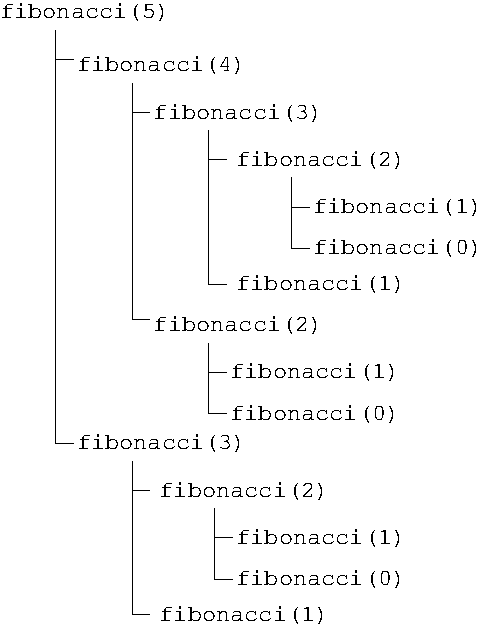
\includegraphics[width=5cm]{recursivite.pdf}}
\end{fig}}
Dans la version récursive, pour calculer {\tt fibonacci(5)},
on calcule d'abord {\tt fibonac\-ci(4)} et {\tt fibonac\-ci(3)}. Pour calculer {\tt fibonacci(4)},
on calcule {\tt fibonac\-ci(3)} et {\tt fibonac\-ci(2)}.
Pour calculer {\tt fibonacci(3)}, on calcule {\tt fibonacci(2)} et {\tt fibonac\-ci(1)}\ldots\ 
Le dérou\-le\-ment du processus ressemble ainsi à un arbre  
(figure \ref{fig:recursivite}). 
On remarque 
que les branches de l'arbre se divise en deux à chaque niveau 
(sauf en bas de l'arbre, {\em ie} à droite sur la figure), 
ce qui traduit le fait que la fonction {\tt fibonacci} s'appelle elle-même deux fois 
à chaque fois qu'elle est invoquée avec {\tt n > 1}. 
Dans cet arbre, on constate par exemple que 
le calcul de {\tt fibonacci(3)} est développé intégralement 2 fois : 
une fois pour le
calul de {\tt fibonacci(4)} et une fois pour lui-même.
En fait, il n'est pas très difficile de montrer que le nombre 
de fois où la fonction calcule {\tt fibonacci(1)} ou {\tt fibonacci(0)} 
({\em ie.} le nombre de feuilles dans l'arbre) est précisément 
$u_n$ ({\tt fibonacci(n)}).
Or la valeur de $u_n$ croît de manière exponentielle avec $n$; ainsi, avec cette version récursive, 
le processus de calcul de {\tt fibonacci(n)} prend un temps qui croît de façon exponentielle
avec {\tt n}.

Dans la version itérative, on ne passe que $(n-1)$ fois dans la boucle.
Ainsi, le processus de calcul itératif de {\tt fibonacci(n)}
prend un temps qui croît de manière linéaire avec {\tt n}.
La différence entre les temps de calcul requis par les 2 méthodes, 
l'une linéaire en $n$ et l'autre augmentant aussi vite que $u_n$ lui-même, 
est donc énorme même pour de petites valeurs de $n$. Par exemple, pour $n = 50$,
il faudra $50$ unités de temps pour la méthode itérative contre $20365011074$ 
(plus de 20 milliards unités de temps !)
pour la méthode récursive. La version itérative sera donc préférée 
à la version récursive dans ce cas là : « il n'y a pas photo » !

\marginpar{\footnotesize\em\vspace*{-1cm}
\begin{fig}[Tours de Hanoï (1)]\label{fig:hanoi}
{\bf Etat initial :}\\
\centerline{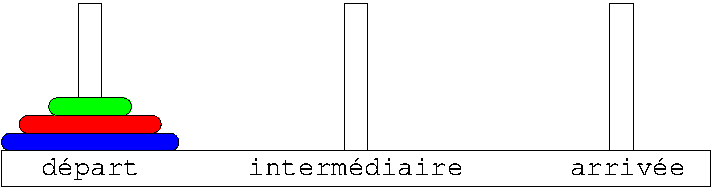
\includegraphics[width=6cm]{hanoi.pdf}}

{\bf Etat final :}\\
\centerline{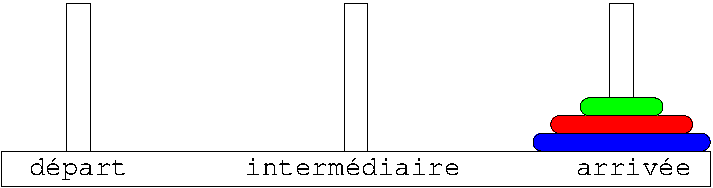
\includegraphics[width=6cm]{hanoi1.pdf}}
\end{fig}

\begin{td}[Tours de Hanoï {\em à la main}]\label{td:hanoi}\index[td]{tours de Hanoï}
Résoudre {\em à la main} le problème des tours de Hanoï à $n$ disques
(voir exemple \ref{ex:hanoi} et figure \ref{fig:hanoi}) successivement 
pour $n=1$, $n=2$, $n=3$ et $n=4$.
\end{td}

\begin{fig}[Tours de Hanoï (2)]\label{fig:hanoi2}
{\bf Etat intermédiaire a:}\\
\centerline{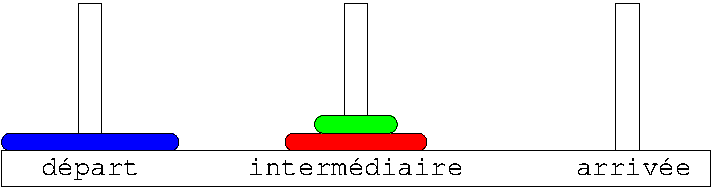
\includegraphics[width=6cm]{hanoi2.pdf}}

\begin{quote}\tt
\begin{center} 
déplacer disque 3 de la tour \\
«~départ » à la tour « arrivée~»
\end{center}
\end{quote}

{\bf Etat intermédiaire b:}\\
\centerline{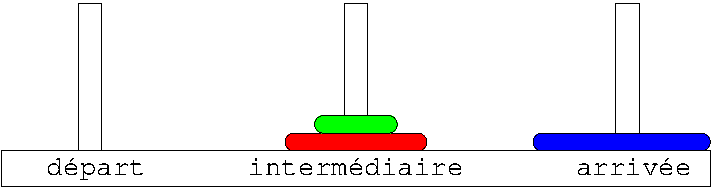
\includegraphics[width=6cm]{hanoi3.pdf}}
\end{fig}
}
Il ne faudrait pas conclure à l'inutilité des processus récursifs en arbre. Pour
les processus opérant sur des structures de données hiérarchiques et non plus sur
des nombres, la récursivité en arbre est un outil naturel et 
puissant\footnote{L'étude des structures de données arborescentes 
est abordée à partir du $5^{\grave eme}$ semestre des enseignements
d'informatique à l'ENIB.}. 
Même pour les calculs numériques, les processus récursifs en arbre peuvent être utiles à la
compréhension et à la conception d'algorithmes. Par exemple, bien que la version
récursive de {\tt fibonacci} soit beaucoup moins efficace que la version
itérative, elle s'obtient presque directement, étant à peine plus qu'une
traduction en \python\ de la définition mathématiques des nombres de Fibonacci.
En revanche, pour formuler la version itérative, il fallait avoir remarqué 
que le calcul pouvait être revu sous la forme d'une itération avec 3 variables;
ce qui est bien moins direct et moins intuitif que la version récursive.

\begin{ex}[Tours de Hanoï]\label{ex:hanoi}
Les « tours de Hanoï » est un jeu imaginé par le mathématicien 
français Édouard Lucas (1842-1891). Il 
consiste à déplacer $n$ disques de diamètres différents d'une 
tour de « départ » à une tour d'« arrivée » en passant par une 
tour « intermédiaire » et ceci en un minimum de coups, 
tout en respectant les règles suivantes :
\begin{itemize}
\item on ne peut déplacer qu'un disque à la fois,
\item on ne peut placer un disque que sur un autre disque 
	plus grand que lui ou sur une tour vide.
\end{itemize}
Dans l'état initial, les $n$ disques sont placés sur la tour
« départ ». Dans l'état final, tous les disques se retrouvent
placés dans le même ordre sur la tour « arrivéee » (figure \ref{fig:hanoi}).
{\em \exo{td:hanoi}}
\end{ex}

\noindent On cherche donc à définir une procédure 
{\tt hanoi(n,depart,intermediaire,arrivee)} qui devra déplacer
{\tt n} disques de la tour {\tt depart} à la tour {\tt arrivee}
en utilisant la tour {\tt intermediaire} comme tour de 
transit.
Numérotons $1,2,3,\ldots,n$ les $n$ disques du plus
petit (numéro $1$) au plus grand (numéro $n$). A un moment donné,
dans la suite des opérations à effectuer, il faudra déplacer le disque 
numéro $n$ (le plus grand, placé initialement en dessous de la 
pile de disques) de la tour « départ » à la tour « arrivée ».
Pour pouvoir effectuer ce déplacement, il faut d'une part qu'il n'y ait plus
aucun disque sur le disque $n$ et d'autre part que la tour « arrivée » soit vide;
en conséquence, il faut que tous les autres disques (de $1$ à $(n-1)$) soient
sur la tour « intermédiaire~» (figure \ref{fig:hanoi2} a). Pour atteindre cet état
intermédiaire, il faut donc déplacer les $(n-1)$ premiers disques de la tour
«~départ » à la tour « intermédiaire~» en utilisant la tour «~arrivée » comme
tour de transit : ce déplacement correspond à l'appel 
{\tt hanoi(n-1,depart,arrivee,intermediaire)}. Une fois réalisé ce déplacement
des $(n-1)$ premiers disques, le disque $n$ peut être déplacé de la tour « départ » 
à la tour « arrivée » (figure \ref{fig:hanoi2} b).
Il ne reste plus qu'à déplacer les $(n-1)$ premiers disques de la tour 
« intermédiaire~» à la tour « arrivée » en utilisant la tour « départ » comme
tour de transit; ces derniers déplacements correspondent
à l'appel {\tt hanoi(n-1,intermediaire,depart,arrivee)}.
\marginpar{\footnotesize\em
\begin{fig}[Récursivité en arbre : {\tt hanoi}]\label{fig:recursivite2}
\begin{py}{5cm}\tt
>>> hanoi(3,'d','i','a')\\
\mbox{}
\end{py}

\centerline{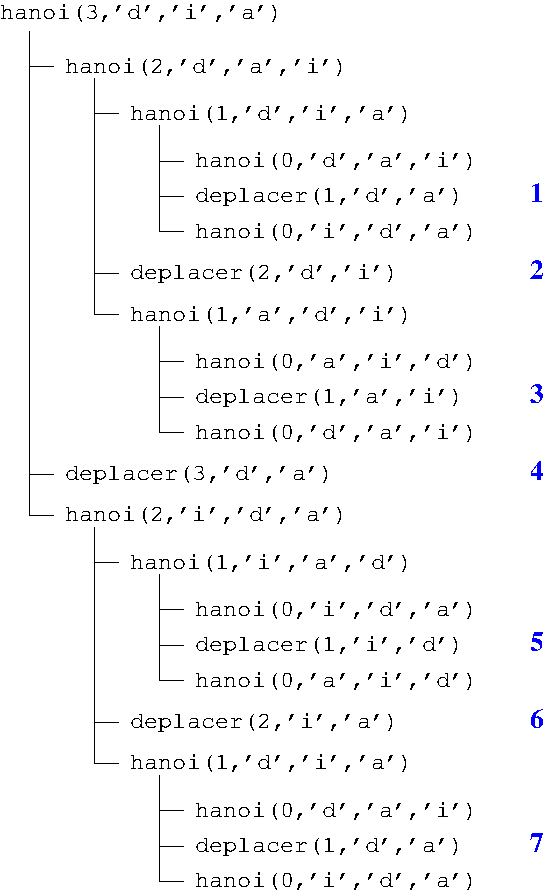
\includegraphics[width=5cm]{recursivite2.pdf}}
\end{fig}
}
On en déduit l'implémentation de la procédure {\tt hanoi} de la page suivante
où le déplacement y est traduit par un simple affichage du type :
{\tt déplacer disque 3 de la tour « départ » à la tour « arrivée »}. Un appel
de cette procédure pour $n = 3$ est donné à titre d'exemple; 
les tours « départ », « intermédiaire~» et « arrivée »
y sont respectivement nommées {\tt 'd'}, {\tt 'i'} et {\tt 'a'}.

\noindent\mbox{}\hspace*{1cm}
\begin{py}{6cm}
\begin{verbatim}
def hanoi(n,gauche,milieu,droit):
    assert type(n) is int
    assert n >= 0
    if n > 0:
        hanoi(n-1,gauche,droit,milieu)
        deplacer(n,gauche,droit)
        hanoi(n-1,milieu,droit,gauche)
    return

def deplacer(n,gauche,droit):
    print('déplacer disque', n,
          'de la tour', gauche, 
          'à la tour', droit)
    return
\end{verbatim}
\end{py}
\hfill
\begin{py}{6cm}
\begin{verbatim}
>>> hanoi(3,'d','i','a')
déplacer disque 1 de la tour d à la tour a
déplacer disque 2 de la tour d à la tour i
déplacer disque 1 de la tour a à la tour i
déplacer disque 3 de la tour d à la tour a
déplacer disque 1 de la tour i à la tour d
déplacer disque 2 de la tour i à la tour a
déplacer disque 1 de la tour d à la tour a
\end{verbatim}
\end{py}
\hspace*{1cm}\mbox{}\vspace*{2mm}

\noindent L'exécution d'un appel à la procédure {\tt hanoi} s'apparente ici encore
à un processus récursif en arbre : les 7 déplacements effectués lors
de l'appel {\tt hanoi(3,'d','i','a')} sont numérotés dans leur ordre d'apparition
sur la figure \ref{fig:recursivite2} (les appels à la fonction {\tt hanoi}
pour {\tt n = 0} ne font rien). Mais toutes les fonctions récursives ne
conduisent pas nécessairement à un processus récursif en arbre 
comme l'exemple de la fonction {\tt factorielle} le montre.

\begin{ex}[Fonction factorielle]\label{ex:factorielle}
La fonction factorielle qui calcule le produit des 
$n$ premiers entiers positifs ($\displaystyle n! = \prod_{k=1}^n k$) 
est simplement définie par la relation de
récurrence :
$$\left\{\begin{array}{l@{\ =\ }ll}
0! & 1 & \\
n! & n\cdot (n-1)! & \forall n \in N^*
\end{array}\right.$$
\end{ex}

\marginpar{\footnotesize\em
\begin{fig}[Récursivité linéaire : {\tt factorielle}]\label{fig:factorielle}
\tt
factorielle(5)\\
(5*factorielle(4))\\
(5*(4*factorielle(3)))\\
(5*(4*(3*factorielle(2))))\\
(5*(4*(3*(2*factorielle(1)))))\\
(5*(4*(3*(2*1))))\\
(5*(4*(3*2)))\\
(5*(4*6))\\
(5*24)\\
120
\end{fig}
}
\noindent\mbox{}\hspace*{1cm}\begin{py}{6cm}
{\bf Version itérative :}\\\tt
def factorielle(n):\\
\mbox{}\ \ \ \ u = 1\\
\mbox{}\ \ \ \ for i in range(2,n+1):\\
\mbox{}\ \ \ \ \ \ \ \ u = u * i\\
\mbox{}\ \ \ \ return u
\end{py}
\hfill
\begin{py}{6cm}
{\bf Version récursive :}\\\tt
def factorielle(n):\\
\mbox{}\ \ \ \ u = 1\\
\mbox{}\ \ \ \ if n > 1:\\
\mbox{}\ \ \ \ \ \ \ \ u = n * factorielle(n-1)\\
\mbox{}\ \ \ \ return u
\end{py}
\hspace*{1cm}\mbox{}\vspace*{2mm}

\noindent On retrouve à gauche la version itérative bien connue. 
A droite, la version récursive est la traduction directe
de la formulation mathématique. Dans la version récursive,
le processus nécessite que l'interpréteur garde une trace des multiplications
à réaliser plus tard (figure \ref{fig:factorielle}). Le processus croît
puis décroît : la croissance se produit lorsque le processus construit une chaîne
d'opérations différées (ici, une chaîne de multiplications différées) et 
la décroissance intervient lorsqu'on peut évaluer les multiplications.
Ainsi, la quantité d'information qu'il faut mémoriser pour effectuer plus tard
les opérations différées croît linéairement avec $n$ : on parle de processus
récursif linéaire. 
\marginpar{\footnotesize\em
\begin{td}[Pgcd et ppcm de 2 entiers (1)]\label{td:pgcd}\index[td]{pgcd et ppcm de 2 entiers}
\begin{enumerate}
\item Définir une fonction récursive qui calcule le plus grand commun 
	diviseur $d$ de 2 entiers $a$ et $b$ : \\
	$\rm{pgcd}(a,b) = \rm{pgcd}(b,a \bmod b) = \ldots \\\ldots = \rm{pgcd}(d,0) = d$.
\item En déduire une fonction qui calcule le plus petit commun multiple $m$ de 2 entiers $a$ et $b$.
\end{enumerate}
\end{td}}
L'interprétation d'une fonction récursive passe donc par une phase 
d'expansion dans lesquels les appels récursifs sont « empilés » jusqu'à 
arriver à un appel de la fonction pour lequel une condition d'arrêt sera 
vérifiée, puis par une phase de contraction dans laquelle les résultats 
des appels précédemment empilés sont utilisés.
Par contre, dans la version itérative, le processus de calcul ne croît ni
ne décroît : à chaque étape, seules les valeurs courantes des variables 
{\tt u} et {\tt i} sont nécessaires (il n'y a pas d'opérations différées)
et le temps requis pour calculer $n!$ augmente linéairement avec $n$
(on passe $n-2$ fois dans la boucle).
\exo{td:pgcd}

Lorsqu'on parle de fonction récursive, on fait référence à une
caractéristique syntaxique : la fonction, dans sa propre définition,
se fait réfèrence à elle-même (elle s'appelle elle-même). 
Mais lorsqu'on parle de processus récursif, linéaire ou en arbre, 
on s'intéresse au déroulement du processus, et non à la syntaxe de 
l'écriture de la fonction. 
Ainsi, une fonction peut avoir une définition récursive mais correspondre à
un processus itératif : c'est le cas de la nouvelle version de la fonction 
{\tt factorielle} ci-dessous.

\noindent\mbox{}\hspace*{1cm}\begin{py}{6cm}
\begin{verbatim}
def factorielle(n):
    u = factIter(n,1,1)
    return u

def factIter(n,i,fact):
    u = fact
    if i < n:
        u = factIter(n,i+1,fact*(i+1))
    return u
\end{verbatim}
\end{py}
\hfill
\begin{py}{6cm}
\begin{verbatim}
factorielle(5)
(factIter(5,1,1))
(factIter(5,2,2))
(factIter(5,3,6))
(factIter(5,4,24))
(factIter(5,5,120))
120
\end{verbatim}
\end{py}
\hspace*{1cm}\mbox{}\vspace*{2mm}

\marginpar{\footnotesize\em\vspace*{-1cm}
\begin{td}[Somme arithmétique]\label{td:somme}\index[td]{suite arithmétique}
\begin{enumerate}
\item Définir une fonction récursive qui calcule la somme des $n$ premiers
	nombres entiers.
	$$s = \sum^{n}_{k=0}k = \frac{n(n+1)}{2}$$
\item Comparer la complexité de cette version avec les versions constante
	et itérative (voir TD \ref{td:implem}).
\end{enumerate}
\end{td}

\begin{td}[Courbes fractales]\label{td:fractal}\index[algo]{courbes fractales}\index[td]{courbes fractales}
On s'intéresse ici aux programmes dont l'exécution produit des dessins
à l'aide de la tortue Logo (voir annexe \ref{logo} page \pageref{logo}).
On consid\`ere la proc\'edure {\tt draw} ci-dessous :

\mbox{}\ \ \begin{py}{7cm}\tt
def draw(n,d):\\
\mbox{}\ \ \ \ assert type(n) is int\\
\mbox{}\ \ \ \ assert n >= 0\\
\mbox{}\ \ \ \ if n == 0: forward(d)\\
\mbox{}\ \ \ \ else:\\
\mbox{}\ \ \ \ \ \ \ \ draw(n-1,d/3.)\\
\mbox{}\ \ \ \ \ \ \ \ left(60)\\
\mbox{}\ \ \ \ \ \ \ \ draw(n-1,d/3.)\\
\mbox{}\ \ \ \ \ \ \ \ right(120)\\
\mbox{}\ \ \ \ \ \ \ \ draw(n-1,d/3.)\\
\mbox{}\ \ \ \ \ \ \ \ left(60)\\
\mbox{}\ \ \ \ \ \ \ \ draw(n-1,d/3.)\\
\mbox{}\ \ \ \ return
\end{py}\\[1mm]
Dessiner le résultat des appels {\tt draw(n,900)} respectivement pour {\tt n = 0},
	{\tt n = 1}, {\tt n = 2} et {\tt n = 3}. A chaque appel, le crayon est 
	initialement en $(0,0)$ avec une direction de $0$.
\end{td}}
\noindent La nouvelle fonction {\tt factorielle} appelle une fonction
auxiliaire {\tt factIter} dont la définition est syntaxiquement récursive
({\tt factIter} s'appelle elle-même). Cette fonction à 3 arguments : l'entier {\tt n} 
dont il faut calculer la factorielle, un compteur {\tt i} initialisé à {\tt 1}
au premier appel de {\tt factIter} par {\tt factorielle} et incrémenté à chaque
nouvel appel, et un nombre {\tt fact} initialisé à {\tt 1} et multiplié
par la nouvelle valeur du compteur à chaque nouvel appel. Le déroulement
d'un appel à {\tt factIter} montre qu'ainsi, à chaque étape, la relation
{\tt (i! == fact)} est toujours vérifiée. La fonction {\tt factIter}
arrête de s'appeler elle-même lorsque {\tt (i == n)} et on a alors 
{\tt (fact == i! == n!)} qui est la valeur recherchée. Ainsi, à chaque étape,
nous n'avons besoin que des valeurs courantes du compteur {\tt i} 
et du produit {\tt fact},
exactement comme dans la version itérative de la fonction {\tt factorielle} :
il n'y a plus de chaîne d'opérations différées comme dans la version récursive
de {\tt factorielle}. Le processus mis en jeu ici est un processus itératif, 
bien que la définition de {\tt factIter} soit récursive.
\exo{td:somme}

Dans la fonction {\tt factIter}, le résultat de l'appel récursif est
retourné par la fonction : on parle alors de récursivité terminale (ou récursivité à droite).
L'exécution d'un tel appel termine l'exécution de la fonction.

\begin{defin}[récursivité terminale]\index[def]{récursivité terminale}\index{fonction!récursivité terminale}
Un appel récursif terminal est un appel récursif dont le résultat est celui 
retourné par la fonction.
\end{defin}

En d'autres termes, si dans le corps d'une fonction, un appel récursif 
est placé de telle façon que son exécution n'est jamais suivi par l'exécution 
d'une autre instruction de la fonction, cet appel est dit récursif
à droite. Si ce n'est pas le cas, on parle de récursivité non terminale ou de récursivité à gauche.
\exo{td:fractal}

\begin{defin}[récursivité non terminale]\index[def]{récursivité non terminale}\index{fonction!récursivité non terminale}
Un appel récursif non terminal est un appel récursif dont le résultat 
n'est pas celui retourné par la fonction.
\end{defin}


%-------------------------------------------------------------------------
\subsection{Fonction récursive ou fonction itérative}\label{sub:recursivite-itérativite}
%-------------------------------------------------------------------------
Quel que soit le problème à résoudre, on a le choix entre l'écriture d'une fonction itérative et celle d'une
fonction récursive. Si le problème admet une décomposition récurrente naturelle, le programme récursif est
alors une simple adaptation de la décomposition choisie. C'est le cas des fonctions {\tt factorielle} et
{\tt fibonacci} par exemple. 
L'approche récursive présente cependant des inconvénients :
certains langages n'admettent pas la récursivité (comme le langage machine !)
et elle est souvent coûteuse en mémoire comme en temps d'exécution. 
On peut pallier ces inconvénients en transformant la fonction récursive 
en fonction itérative : c'est toujours possible.

Considérons une procédure {\tt f} à récursivité terminale écrite en pseudo-code :

\noindent\mbox{}\hspace*{1cm}\begin{py}{4cm}
\begin{verbatim}
def f(x):
    if cond: arret
    else:
        instructions
        f(g(x))
    return
\end{verbatim}
\end{py}
\hfill
\begin{py}{9cm}
{\tt x} représente ici la liste des arguments de la fonction,
{\tt cond} une condition portant sur {\tt x}, 
{\tt instructions} un bloc d'instructions qui constituent
le traitement de base de la fonction {\tt f}, 
{\tt g(x)} une transformation des arguments et {\tt arret}
l'instruction de terminaison (clause d'arrêt) de la récurrence.
\end{py}

\vspace*{2mm}

\noindent Elle est équivalente à la procédure itérative suivante :\label{methode:recursivite}

\noindent\mbox{}\hspace*{1cm}\begin{py}{4cm}
\begin{verbatim}
def f(x):
    while not cond: 
        instructions
        x = g(x)
    arret
    return
\end{verbatim}
\end{py}

\vspace*{2mm}

\noindent Illustrons cette transformation à l'aide de la fonction qui calcule le {\tt pgcd} de 2 entiers.

\noindent\mbox{}\hspace*{1cm}\begin{py}{4cm}
\begin{verbatim}
def pgcd(a,b):
    if b == 0: return a
    else: 
        pass # ne fait rien
        return pgcd(b,a%b)

>>> pgcd(12,18)
6
\end{verbatim}
\end{py}
\hfill
\begin{py}{4cm}\tt
\begin{tabular}[t]{|l@{ $\rightarrow$ }l|}
\hline
x & a,b\\
cond & b == 0\\
arret & return a\\
instructions & {\rm pass}\\
x = g(x) & a,b = b,a\%b\\
\hline
\end{tabular}
\end{py}
\hfill
\begin{py}{4cm}
\begin{verbatim}
def pgcd(a,b):
    while not (b == 0):
        pass
        a,b = b,a%b
    return a

>>> pgcd(12,18)
6
\end{verbatim}
\end{py}

\vspace*{2mm}

La méthode précédente ne s'applique qu'à la récursivité terminale.
Une méthode générale existe pour transformer une fonction récursive
quelconque en une fonction itérative équivalente. En particulier,
elle est mise en \oe uvre dans les compilateurs car le langage machine 
n'admet pas la récursivité. Cette méthode générale fait appel à la notion 
de pile (section \ref{pilefile} page \pageref{pilefile}) pour sauvegarder
le contexte des appels récursifs. On l'illustrera dans le cas particulier 
du tri d'une liste par la méthode
du tri rapide (section \ref{sub:triRapide} page \pageref{sub:triRapide}).

%-------------------------------------------------------------------------
\newpage
\setlength{\textwidth}{25cm}
\setlength{\textheight}{16cm}
\setlength{\marginparwidth}{0cm}
\setlength{\marginparsep}{0cm}
\setlength{\linewidth}{25cm}
\setlength{\oddsidemargin}{0cm}
\setlength{\evensidemargin}{0cm}
\setlength{\topmargin}{-0.75cm}

\section{Exercices complémentaires}
%-------------------------------------------------------------------------

%-------------------------------------------------------------------------
\subsection{Connaître}
%-------------------------------------------------------------------------
\begin{td}[QCM (3)]\label{td:qcm3}\index{evaluation@évaluation!contrôle d'attention}
\index{fonction!qcm}\index[td]{contrôle d'attention} (un seul item correct par question)
\em
\begin{enumerate}
\item La réutilisabilité d'un algorithme est son aptitude
	\begin{enumerate}
	\item à utiliser de manière optimale les ressources du matériel qui l'exécute
	\item à se protéger de conditions anormales d'utilisation
	\item à résoudre des tâches équivalentes à celle pour laquelle il a été conçu
	\item à réaliser exactement la tâche pour laquelle il a été conçu
	\end{enumerate}

\item L'encapsulation est l'action
	\begin{enumerate}
	\item de mettre une chose dans une autre
	\item de fermer une chose par une autre
	\item de substituer une chose par une autre
	\item de remplacer une chose par une autre
	\end{enumerate}
	
\item Une fonction est un bloc d'instructions nommé et paramétré 
	\begin{enumerate}
	\item qui ne peut pas retourner plusieurs valeurs
	\item qui ne peut pas contenir d'instructions itératives
	\item qui retourne une valeur
	\item qui ne retourne pas de valeur
	\end{enumerate}

\item Les paramètres d'entrée d'une fonction sont
	\begin{enumerate}
	\item les arguments nécessaires pour effectuer le traitement associé à la fonction
	\item les valeurs obtenues après avoir effectué le traitement associé à la fonction
	\item des grandeurs invariantes pendant l'exécution de la fonction
	\item des variables auxiliaires définies dans le corps de la fonction
	\end{enumerate}
	
\item Les préconditions d'une fonction sont des conditions à respecter 
	\begin{enumerate}
	\item par les paramètres de sortie de la fonction
	\item pendant toute l'exécution de la fonction
	\item par les paramètres d'entrée de la fonction
	\item pour pouvoir compiler la fonction
	\end{enumerate}
	
\item La description d'une fonction décrit
	\begin{enumerate}
	\item ce que fait la fonction
	\item comment fait la fonction
	\item pourquoi la fonction le fait 
	\item où la fonction le fait
	\end{enumerate}
	
\item Le jeu de tests d'une fonction est 
	\begin{enumerate}
	\item un ensemble d'exercices à résoudre
	\item un ensemble d'exceptions dans le fonctionnement de la fonction
	\item un ensemble caractéristiques d'entrées-sorties associées
	\item un ensemble de recommandations dans l'utilisation de la fonction
	\end{enumerate}

\item En {\sc Python}, l'instruction {\tt assert} permet de 
	\begin{enumerate}
	\item tester une précondition
	\item imposer une instruction
	\item paramétrer une fonction
	\item tester un test du jeu de tests
	\end{enumerate}

\item La validité d'une fonction est son aptitude à réaliser exactement 
	la tâche pour laquelle elle a été conçue. Plus concrètement,
	\begin{enumerate}
	\item la fonction doit vérifier impérativement ses préconditions
	\item la fonction doit être correctement paramétrée
	\item l'implémentation de la fonction doit être conforme aux jeux de tests
	\item l'utilisation de la fonction doit être conviviale
	\end{enumerate}

\item Le passage des paramètres par valeur consiste à copier
	\begin{enumerate}
	\item la valeur du paramètre formel dans le paramètre effectif correspondant
	\item la référence du paramètre effectif dans le paramètre formel correspondant
	\item la référence du paramètre formel dans le paramètre effectif correspondant
	\item la valeur du paramètre effectif dans le paramètre formel correspondant
	\end{enumerate}
	
\item Un appel récursif est un appel 
	\begin{enumerate}
	\item dont l'exécution est un processus récursif
	\item dont l'exécution est un processus itératif
	\item dont le résultat est retourné par la fonction
	\item d'une fonction par elle-même
	\end{enumerate}	
\end{enumerate}
\end{td}


%-------------------------------------------------------------------------
\subsection{Comprendre}
%-------------------------------------------------------------------------
\begin{td}[Passage des paramètres]\label{td:passage}\index{fonction!passage par valeur}\index[td]{passage par valeur}
\em
On considère les fonctions {\tt f}, {\tt g} et {\tt h} suivantes :

\begin{center}
\begin{py}{4cm}
\begin{verbatim}
def f(x):
    y = x + 2
    return y
\end{verbatim}
\end{py}\hspace*{1cm}
\begin{py}{4cm}
\begin{verbatim}
def g(z):
    v = 2*f(z)
    return v
\end{verbatim}
\end{py}\hspace*{1cm}
\begin{py}{4cm}
\begin{verbatim}
def h(a):
    b = g(f(a))
    return b
\end{verbatim}
\end{py}
\end{center}

Quels sont les algorithmes équivalents (algorithmes où il n'y a plus 
d'appels aux fonctions {\tt f}, {\tt g} et {\tt h}) aux appels suivants :
\vspace*{2mm}

\begin{minipage}{3.5cm}
\begin{enumerate}
\item {\tt u = f(2)}
\end{enumerate}
\end{minipage}
\hfill
\begin{minipage}{3.5cm}
\begin{enumerate}\setcounter{enumi}{1}
\item {\tt u = f(t)}
\end{enumerate}
\end{minipage}
\hfill
\begin{minipage}{3.5cm}
\begin{enumerate}\setcounter{enumi}{2}
\item {\tt u = g(2)}
\end{enumerate}
\end{minipage}
\hfill
\begin{minipage}{3.5cm}
\begin{enumerate}\setcounter{enumi}{3}
\item {\tt u = g(t)}
\end{enumerate}
\end{minipage}\hfill
\begin{minipage}{3.5cm}
\begin{enumerate}\setcounter{enumi}{4}
\item {\tt u = h(2)}
\end{enumerate}
\end{minipage}
\hfill
\begin{minipage}{3.5cm}
\begin{enumerate}\setcounter{enumi}{5}
\item {\tt u = h(t)}
\end{enumerate}
\end{minipage}

\end{td}

\begin{td}[Portée des variables (2)]\label{td:portee2}\index{variable!portée}\index[td]{portée des variables}
\em
On considère les fonctions {\tt f}, {\tt g} et {\tt h} suivantes :
\begin{center}
\begin{py}{4cm}
\begin{verbatim}
def f(x):
    x = x + 2
    print('f', x)
    return x
\end{verbatim}
\end{py}\hspace*{1cm}
\begin{py}{4cm}
\begin{verbatim}
def g(x):
    x = 2*f(x)
    print('g', x)
    return x
\end{verbatim}
\end{py}\hspace*{1cm}
\begin{py}{4cm}
\begin{verbatim}
def h(x):
    x = g(f(x))
    print('h', x)
    return x
\end{verbatim}
\end{py}
\end{center}

Qu'affichent les appels suivants ?
\vspace*{2mm}

\begin{minipage}[t]{4cm}
\begin{enumerate}
\item 

\begin{py}{4cm}
\begin{verbatim}
>>> x = 5
>>> print(x)

>>> x = x + 2
>>> print(x)

>>> x = 2 * (x + 2)
>>> print(x)

\end{verbatim}
\end{py}
\end{enumerate}
\end{minipage}
\hfill
\begin{minipage}[t]{4cm}
\begin{enumerate}\setcounter{enumi}{1}
\item 

\begin{py}{4cm}
\begin{verbatim}
>>> x = 5
>>> print(x)

>>> y = f(x)
>>> print(x, y)

>>> z = 2*f(y)
>>> print(x, y, z)

\end{verbatim}
\end{py}
\end{enumerate}
\end{minipage}
\hfill
\begin{minipage}[t]{4cm}
\begin{enumerate}\setcounter{enumi}{2}
\item 

\begin{py}{4cm}
\begin{verbatim}
>>> x = 5
>>> print(x)

>>> z = 2*f(f(x))
>>> print(x, z)

\end{verbatim}
\end{py}
\end{enumerate}
\end{minipage}
\hfill
\begin{minipage}[t]{4cm}
\begin{enumerate}\setcounter{enumi}{3}
\item 

\begin{py}{4cm}
\begin{verbatim}
>>> x = 5
>>> print(x)

>>> f(x)

>>> print(x)

>>> g(x)

>>> print(x)

>>> h(x)

>>> print(x)

\end{verbatim}
\end{py}


\end{enumerate}
\end{minipage}
\end{td}


%-------------------------------------------------------------------------
\subsection{Appliquer}
%-------------------------------------------------------------------------
\begin{td}[Suite géométrique]\label{td:geometrie}\index[algo]{suites numériques}\index[td]{suite
géométriques}
\em
Définir une fonction récursive qui calcule la somme des $n$ premiers termes 
d'une suite géométrique $u_k = ab^k$.
\end{td}

\begin{td}[Puissance entière]\label{td:puissance}\index[algo]{fonction puissance}\index[td]{fonction puissance}
\em
Définir une fonction récursive qui calcule la puissance entière $p = x^n$ 
d'un nombre entier $x$.
\end{td}

\begin{td}[Coefficients du binôme]\label{td:binome}\index[algo]{coefficients du binôme}\index[td]{coefficients du binôme}
\em
Définir une fonction récursive qui calcule les coefficients du binôme 
$\displaystyle (a+b)^n = \sum_{k=0}^n \frac{n!}{k!(n-k)!}a^{n-k}b^k$.
\end{td}

\begin{td}[Fonction d'Ackerman]\label{td:ackerman}\index[algo]{fonction d'Ackerman}\index[td]{fonction d'Ackerman}\index{{{\sc Ackerman}}}
\em
Définir une fonction récursive qui calcule la fonction d'Ackerman : 
$$
{f : N^2 \rightarrow N}\ 
\left\{\begin{array}{lll}
f{(0,n)} & = & n+1\\
f{(m,0)} & = & f{(m-1,1)}\mbox{\ si\ } m > 0\\
f{(m,n)} & = & f{(m-1,f{(m,n-1)})}\mbox{\ si\ } m > 0, n > 0
\end{array}\right.
$$
\end{td}

%-------------------------------------------------------------------------
\subsection{Analyser}
%-------------------------------------------------------------------------

\begin{td}[Addition binaire]\label{td:addition2}\index[algo]{opérations binaires}\index[td]{addition binaire}
\em
Définir une fonction {\tt add2} qui effectue l'addition binaire de 2 
entiers $a$ et $b$ (le nombre de bits n'est pas limité {\em a priori}).\\
Exemple : $(0101)_2 + (10011)_2 = (11000)_2$

\begin{py}{7cm}
\begin{verbatim}
# add2(a,b)
>>> add2([1,0],[1,0,1,1])
[1, 1, 0, 1]
>>> add2([1,0,1,1],[1,0])
[1, 1, 0, 1]
>>> add2([1,1],[1,1])
[1, 1, 0]
\end{verbatim}
\end{py}
\end{td}

\begin{td}[Complément à 2]\label{td:complement2}\index[td]{complément à 2}
\em
Définir une fonction {\tt neg2} qui détermine le complément à 2 en binaire 
d'un entier $n$ codé sur $k$ bits.
	$$(011100)_2 \rightarrow (100100)_2\ :\ \begin{array}[t]{lrr} 
	  & (011100)_2\\
	\hline
	  & (100011)_2\\
	+ & (000001)_2\\
	\hline
	= & (100100)_2
	\end{array}$$

	\begin{py}{7cm}
	\begin{verbatim}
	# neg2(code)
	>>> neg2([0,0,0,1,0,1,1,1])
	[1, 1, 1, 0, 1, 0, 0, 1]
	>>> neg2([1, 1, 1, 0, 1, 0, 0, 1])
	[0, 0, 0, 1, 0, 1, 1, 1]
	>>> for a in [0,1]:
	...    for b in [0,1]:
	...        for c in [0,1]:
	...            add2([a,b,c],neg2([a,b,c]))
	[0, 0, 0]
	[1, 0, 0, 0]
	[1, 0, 0, 0]
	[1, 0, 0, 0]
	[1, 0, 0, 0]
	[1, 0, 0, 0]
	[1, 0, 0, 0]
	[1, 0, 0, 0]
	\end{verbatim}
	\end{py}
\end{td}

\begin{td}[Codage-décodage des réels]\label{td:ieee754}\index[algo]{codage des réels}\index[td]{codage des réels}\index{norme IEEE 754}
\em
\begin{enumerate}
\item Définir une fonction {\tt ieee} qui code
	un nombre réel $x$ selon la norme \ieee\ 754 simple précision
	(\href{http://www.ieee.org}{\ieee} : Institute of Electrical and Electronics Engineers).
	$$x = (-1)^s\cdot (1+m)\cdot 2^{(e-127)}$$
	On pourra vérifier les résultats obtenus avec la fonction {\tt ieee}
	sur le site
	\href{http://babbage.cs.qc.edu/IEEE-754/Decimal.html}{\tt http\char`://babbage.cs.qc.edu/IEEE-754/Decimal.html} .

	\begin{py}{7cm}
	\begin{verbatim}
	# ieee(x)
	>>> ieee(0.0)
	[0, 0, 0, 0, 0, 0, 0, 0, 0, 0, 0, 0, 0, 0, 0, 0, 0, 0, 0, 0, 0, 0, 0, 0, 0, 0, 0, 0, 0, 0, 0, 0]
	>>> ieee(0.625)
	[0, 0, 1, 1, 1, 1, 1, 1, 0, 0, 1, 0, 0, 0, 0, 0, 0, 0, 0, 0, 0, 0, 0, 0, 0, 0, 0, 0, 0, 0, 0, 0]
	>>> ieee(3.1399998664855957)
	[0, 1, 0, 0, 0, 0, 0, 0, 0, 1, 0, 0, 1, 0, 0, 0, 1, 1, 1, 1, 0, 1, 0, 1, 1, 1, 0, 0, 0, 0, 1, 0]
	>>> ieee(-4573.5)
	[1, 1, 0, 0, 0, 1, 0, 1, 1, 0, 0, 0, 1, 1, 1, 0, 1, 1, 1, 0, 1, 1, 0, 0, 0, 0, 0, 0, 0, 0, 0, 0]
	\end{verbatim}
	\end{py}
	\vspace*{1mm}
	
\item Définir une fonction {\tt real} qui décode un nombre réel $x$ 
	codé selon la norme IEEE 754 simple précision.
	$$x = (-1)^s\cdot (1+m)\cdot 2^{(e-127)}$$

	\begin{py}{7cm}
	\begin{verbatim}
	# real(code)
	>>> real(ieee(0.625))
	0.625
	>>> real(ieee(3.1399998664855957))
	3.1399998664855957
	>>> real(ieee(-4573.5))
	-4573.5
	\end{verbatim}
	\end{py}
\end{enumerate}
\end{td}

\begin{td}[Intégration numérique]\label{td:integration}\index[algo]{intégration numérique}\index[td]{intégration numérique}
\em
Soit $f(x)$ une fonction continue de $R \rightarrow R$ à intégrer sur $[a,b]$ 
(on supposera que $f$ à toutes les bonnes propriétés mathématiques pour être
intégrable sur l'intervalle considéré). On cherche à calculer son intégrale
$\displaystyle I = \int_a^b f(x)dx$ qui représente classiquement l'aire
comprise entre la courbe représentative de $f$ et les droites d'équations 
$x=a$, $x=b$ et $y=0$. Les méthodes d'intégration numérique (méthode des rectangles, 
méthode des trapèzes et méthode de Simpson) consistent 
essentiellement à trouver une bonne approximation de cette aire.
$$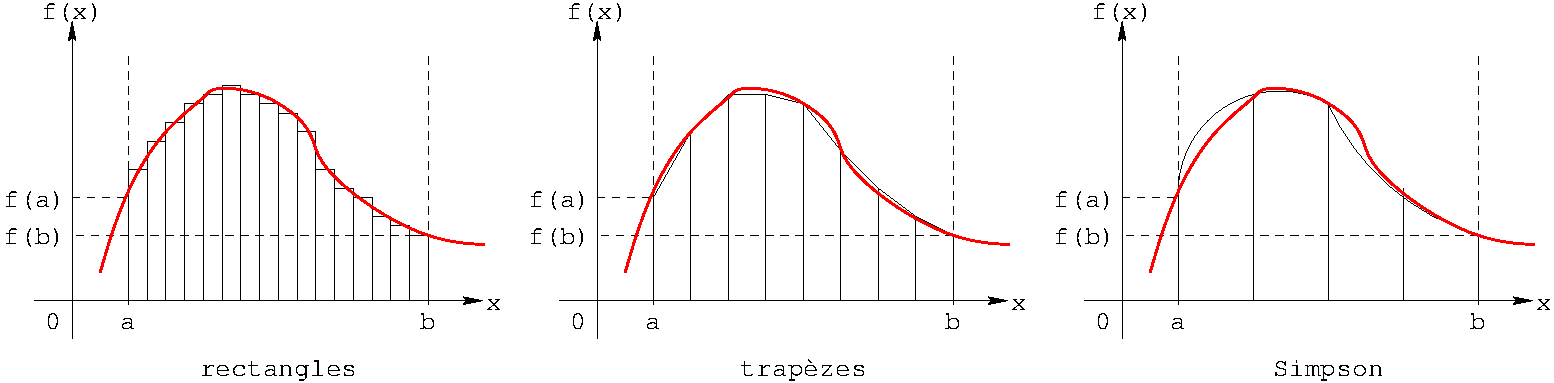
\includegraphics[width=14cm]{integrale.pdf}$$

On testera ces différentes méthodes avec la fonction $f(x) = \sin(x)$ sur $[0,\pi]$.
\begin{enumerate}
\item Méthode des rectangles : subdivisons l'intervalle d'intégration de
	longueur $b-a$ en $n$ parties égales de longueur 
	$\displaystyle\Delta x = \frac{b-a}{n}$. Soient $x_1$, $x_2$, \ldots,
	$x_n$ les points milieux de ces $n$ intervalles. Les $n$ rectangles
	formés avec les ordonnées correspondantes ont pour surface $f(x_1)\Delta
	x$, $f(x_2)\Delta x$, \ldots, $f(x_n)\Delta x$. L'aire sous la courbe 
	est alors assimilée à la somme des aires de ces rectangles, soit 
	$$\displaystyle I = \int_a^b f(x)dx \approx
	\left(f(x_1)+f(x_2)+\cdots+f(x_n)\right)\Delta x$$ 
	C'est la formule dite
	des rectangles qui repose sur une approximation par une fonction {\em en
	escalier}.
	
	Ecrire une fonction {\tt rectangle\_integration} qui calcule l'intégrale définie $I$ d'une fonction 
	$f$ sur $[a,b]$ à l'ordre $n$ par la méthode des rectangles.
	
\item Méthode des trapèzes : subdivisons l'intervalle d'intégration de
	longueur $b-a$ en $n$ parties égales de longueur 
	$\displaystyle\Delta x = \frac{b-a}{n}$. Les abscisses des points ainsi
	définis sont
	$a$, $x_1$, $x_2$, \ldots, $x_{n-1}$, $b$ et les trapèzes construits sur ces
	points et les ordonnées correspondantes ont pour aire 
	$\displaystyle \frac{\Delta x}{2}\left(f(a) + f(x_1)\right)$,
	$\displaystyle \frac{\Delta x}{2}\left(f(x_1) + f(x_2)\right)$,
	\ldots,
	$\displaystyle \frac{\Delta x}{2}\left(f(x_{n-1}) + f(b)\right)$.
	L'aire sous la courbe est alors assimilée à la somme des aires de ces 
	trapèzes, soit
	$$\displaystyle I = \int_a^b f(x)dx \approx
	\left(\frac{f(a)+f(b)}{2} + f(x_1) + f(x_2) + \cdots + f(x_{n-1})\right)
	\Delta x$$
	C'est la formule dite des trapèzes.
	
	Ecrire une fonction {\tt trapezoid\_integration} qui calcule l'intégrale définie $I$ d'une fonction 
	$f$ sur $[a,b]$ à l'ordre $n$ par la méthode des trapèzes.
	
\item Méthode de Simpson : divisons l'intervalle d'intégration $[a,b]$ en un nombre 
	$n$ pair d'intervalles dont la longueur est 
	$\displaystyle\Delta x = \frac{b-a}{n}$. 
	Dans les 2 premiers intervalles d'extrémités $a$, $x_1$ et $x_2$, on approche 
	la courbe représentative de $f$ par une parabole d'équation 
	$y = \alpha x^2 + \beta x + \gamma$ passant par les points $A(a,f(a))$, 
	$A_1(x_1,f(x_1))$ et $A_2(x_2,f(x_2))$ de la courbe. Dans les 2 intervalles 
	suivants, on approche la courbe par une autre parabole d'équation similaire, 
	passant par les points $A_2$, $A_3$ et $A_4$, et ainsi de suite.
	On obtient ainsi une courbe formée de $n$ portions de parabole et
	l'aire déterminée par ces portions de parabole est une approximation de l'aire $I$
	cherchée.
	
	L'intégration de l'équation de la parabole $y = \alpha x^2 + \beta x + \gamma$ sur
	$\displaystyle \left[-\Delta x,\Delta x\right]$ donne 
	$$S = \int_{-\Delta x}^{\Delta x} (\alpha x^2 + \beta x + \gamma)dx = 
	\frac{2}{3}\alpha(\Delta x)^3 + 2\gamma(\Delta x)$$
	où les constantes $\alpha$ et $\gamma$ sont déterminées en écrivant que les points
	$(-\Delta x,y_0)$, $(0,y_1)$ et $(\Delta x,y_2)$ satisfont l'équation de la parabole.
	On obtient ainsi :
	$$\left|\begin{array}{l@{\ =\ }l}
	y_0 & \alpha(-\Delta x)^2 + \beta(-\Delta x) + \gamma\\
	y_1 & \gamma\\
	y_2 & \alpha(\Delta x)^2 + \beta(\Delta x) + \gamma
	\end{array}\right.
	\Rightarrow
	\left|\begin{array}{l@{\ =\ }l}
	\alpha & \displaystyle \frac{y_0 - 2y_1 + y_2}{2(\Delta x)^2} \\
	\beta  & \displaystyle \frac{y_2-y_0}{2(\Delta x)}\\
	\gamma & \displaystyle y_1
	\end{array}\right.$$
	et $\displaystyle S = \frac{\Delta x}{3}(y_0+4y_1+y_2)$.
	
	Par suite, il vient :
	$\displaystyle\left|\begin{array}{l@{\ =\ }l}
	S_1     & \displaystyle \frac{\Delta x}{3}(y_0 + 4y_1 + y_2)\\
	S_2     & \displaystyle \frac{\Delta x}{3}(y_2 + 4y_3 + y_4)\\
	S_3     & \displaystyle \frac{\Delta x}{3}(y_4 + 4y_5 + y_6)\\
	\vdots  \\
	\displaystyle S_{n/2} & \displaystyle \frac{\Delta x}{3}(y_{n-2} + 4y_{n-1} + y_n)
	\end{array}\right.$ 
	
	d'où
	$$I = \int_a^b f(x)dx \approx \frac{\Delta x}{3}
	\left(f(a) + 4\sum_{i=1,3,5...}^{n-1}f(x_i) + 2\sum_{i=2,4,6...}^{n-2}f(x_i) + f(b)\right)$$
	
	C'est la formule dite de Simpson qui repose sur une approximation de $f$ 
	par des arcs de parabole.\index{{{\sc Simpson}}}

	Ecrire une fonction {\tt simpson\_integration} qui calcule l'intégrale définie $I$ d'une fonction 
	$f$ sur $[a,b]$ à l'ordre $n$ par la méthode de Simpson.
\end{enumerate}
\end{td}

\begin{td}[Tracés de courbes paramétrées]\label{td:traces}\index[algo]{courbes paramétrées}\index[td]{courbes paramétrées}
\em
Une courbe paramétrée dans le plan est une courbe où l'abscisse $x$ et l'ordonnée $y$
sont des fonctions d'un paramètre qui peut être le temps $t$ ou un angle $\theta$ par exemple.
La courbe se présente donc sous la forme $x = f(t), y= g(t)$. Les tableaux ci-dessous en donnent quelques
exemples.

{\small
\noindent\begin{tabular}[t]{|ll|}
\hline
droite & $x = x_0 + \alpha t$\\
       & $y = y_0 + \beta t$\\
\hline
cercle & $x = x_0 + r\cos(\theta)$\\
       & $y = y_0 + r\sin(\theta)$\\
\hline
ellipse & $x = x_0 + a\cos(\phi)$\\
        & $y = y_0 + b\cos(\phi)$ \\
\hline
hyperbole & $\displaystyle x = x_0 + \frac{a}{\cos(\theta)}$ \\
          & $ y = y_0 + b \tan(\theta)$\\
\hline
\end{tabular}
\hfill
\begin{tabular}[t]{|ll|}
\hline
cycloïde & $x = x_0 + r(\phi - \sin(\phi))$\\
       & $y = y_0 + r(1 - \cos(\phi))$\\
\hline
épicycloïde & $\displaystyle x = x_0 + (R+r)\cos(\theta) - r\cos\left(\frac{R+r}{r}\cdot\theta\right)$\\
       & $\displaystyle y = y_0 + (R+r)\sin(\theta) - r\sin\left(\frac{R+r}{r}\cdot\theta\right)$\\
\hline
hypercycloïde & $\displaystyle x = x_0 + (R-r)\cos(\theta) + r\cos\left(\frac{R-r}{r}\cdot\theta\right)$\\
        & $\displaystyle x = y_0 + (R-r)\sin(\theta) + r\sin\left(\frac{R-r}{r}\cdot\theta\right)$ \\
\hline
\end{tabular}
\hfill
\begin{tabular}[t]{|ll|}
\hline
limaçon de Pascal & $x = x_0 + (a\cos(\theta) + b)\cos(\theta)$\\
                  & $y = y_0 + (a\cos(\theta) + b)\sin(\theta)$\\
\hline
spirale logarithmique & $\displaystyle x = x_0 + ke^\theta\cos(\theta)$\\
                      & $\displaystyle y = y_0 + ke^\theta\sin(\theta)$\\
\hline
\end{tabular}
}


$$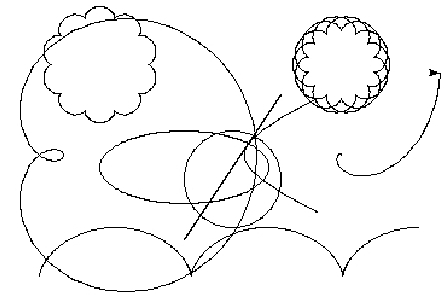
\includegraphics[width=10cm]{param2.jpg}$$



Ecrire une fonction {\tt drawCurve} qui permettent le tracé de telles courbes paramétrées.
On utilisera les instructions {\em à la {\sc Logo}} pour réaliser ces tracés
(voir annexe \ref{logo} page \pageref{logo}).
\end{td}


%-------------------------------------------------------------------------
\subsection{Solutions des exercices}\label{sub:solutions}
%-------------------------------------------------------------------------
\begin{description}
\item[TD \ref{td:qcm3} :] QCM (3).\\
	Les bonnes réponses sont extraites directement de ce document.\\
	1c, 2a, 3c, 4a, 5c, 6a, 7c, 8a, 9c, 10d, 11d

\item[TD \ref{td:passage} :] Passage des paramètres.\\
\begin{minipage}[t]{6cm}
\begin{enumerate}

\item {\tt u = f(t)}

\begin{py}{6cm}
\begin{verbatim}
x = t
y = x + 2
tmp = y
del x, y
u = tmp
del tmp
\end{verbatim}
\end{py}
\end{enumerate}
\end{minipage}
\hfill
\begin{minipage}[t]{6cm}
\begin{enumerate}\setcounter{enumi}{1}

\item {\tt u = g(t)}

\begin{py}{6cm}
\begin{verbatim}
z = t
x = z
y = x + 2
tmp = y
del x, y
v = 2*tmp
tmp = v
del v, z
u = tmp
del tmp
\end{verbatim}
\end{py}
\end{enumerate}
\end{minipage}
\hfill
\begin{minipage}[t]{6cm}
\begin{enumerate}\setcounter{enumi}{2}

\item {\tt u = h(t)}

\begin{py}{6cm}
\begin{verbatim}
a = t
x = a
y = x + 2
tmp = y
del x, y
z = tmp
del tmp
x = z
y = x + 2
tmp = y
del x, y
v = 2*tmp
tmp = v
del v, z
b = tmp
del tmp
tmp = b
del a, b
u = tmp
del tmp
\end{verbatim}
\end{py}

\end{enumerate}
\end{minipage}

\item[TD \ref{td:portee2} :] Portée des variables (2).\\
\begin{minipage}[t]{6cm}
\begin{enumerate}
\item 

\begin{py}{6cm}
\begin{verbatim}
>>> x = 5
>>> x
5
>>> x = x + 2
>>> x
7
>>> x = 2*(x+2)
>>> x
18
\end{verbatim}
\end{py}
\end{enumerate}
\end{minipage}
\hfill
\begin{minipage}[t]{6cm}
\begin{enumerate}\setcounter{enumi}{1}
\item 

\begin{py}{6cm}
\begin{verbatim}
>>> x = 5
>>> x
5
>>> y = f(x)
f 7
>>> x, y
(5, 7)
>>> z = 2*f(y)
f 9
>>> x, y, z
(5, 7, 18)
\end{verbatim}
\end{py}
\end{enumerate}
\end{minipage}
\hfill
\begin{minipage}[t]{6cm}
\begin{enumerate}\setcounter{enumi}{2}
\item 

\begin{py}{6cm}
\begin{verbatim}
>>> x = 5
>>> x
5
>>> z = 2*f(f(x))
f 7
f 9
>>> x, z
(5, 18)
\end{verbatim}
\end{py}
\end{enumerate}
\end{minipage}


\begin{minipage}[t]{6cm}
\begin{enumerate}\setcounter{enumi}{3}
\item 

\begin{py}{6cm}
\begin{verbatim}
>>> x = 5
>>> x
5
>>> f(x)
f 7
7
>>> x
5
>>> g(x)
f 7
g 14
14
>>> x
5
>>> h(x)
f 7
f 9
g 18
h 18
18
>>> x
5
\end{verbatim}
\end{py}
\end{enumerate}
\end{minipage}
\end{description}

\begin{minipage}[t]{10cm}
\begin{description}
\item[TD \ref{td:geometrie} :] Suite géométrique.\index[algo]{suites numériques}
	$$s = \sum_{k=0}^{n} a\cdot b^k = a\frac{b^{n+1}-1}{b-1}$$
	\begin{py}{14cm}
	\begin{verbatim}
	def sommeGeometrique(a,b,n):
	    """
	    s = sommeGeometrique(a,b,n)
	    est la somme des n premiers termes d'une suite
	    géométrique a*b^k (k in [0,n])
	    """
	    assert type(n) is int and n >= 0
	    if n == 0: s = 1
	    else: s = sommeGeometrique(a,b,n-1) + (a * b**n)
	    return s
	\end{verbatim}
	\end{py}
\end{description}
\end{minipage}
\hfill
\begin{minipage}[t]{10cm}
\begin{description}
\item[TD \ref{td:puissance} :] Puissance entière.\index[algo]{fonction puissance}
	$$p = x^n$$
	\begin{py}{14cm}
	\begin{verbatim}
	def puissance(x,n):
	    """"
	    y = puissance(x,n)
	    est la puissance entière de x de degré n
	    """
	    assert type(n) is int and n >= 0
	    if n == 0: p = 1
	    else: p = x*puissance(x,n-1)
	    return p
	\end{verbatim}
	\end{py}
\end{description}
\end{minipage}

\begin{description}
\item[TD \ref{td:binome} :]Coefficients du binôme.\index[algo]{coefficients du binôme}
	$$(a+b)^n = \sum_{k=0}^n \frac{n!}{k!(n-k)!}x^{n-k}y^k$$
	
	\begin{py}{14cm}
	\begin{verbatim}
	def coefficientBinome(n,p):
	    """
	    c = coefficientBinome(n,p)
	    est le p-ième coefficient du binôme (a+b)**n
	    """
	    assert type(n) is int and type(p) is int
	    assert n >= 0 and p >= 0 and p <= n
	    if p == 0 or n == 0 or n == p: c = 1
	    else: c = coefficientBinome(n-1,p) + coefficientBinome(n-1,p-1)
	    return c
	\end{verbatim}
	\end{py}

\item[TD \ref{td:ackerman} :] Fonction d'Ackerman.\index[algo]{fonction d'Ackerman}
	$$
	{f : N^2 \rightarrow N}\ 
	\left\{\begin{array}{lll}
	f{(0,n)} & = & n+1\\
	f{(m,0)} & = & f{(m-1,1)}\mbox{\ si\ } m > 0\\
	f{(m,n)} & = & f{(m-1,f{(m,n-1)})}\mbox{\ si\ } m > 0, n > 0
	\end{array}\right.
	$$

	\begin{py}{14cm}
	\begin{verbatim}
	def ackerman(m,n):
	    """
	    y = ackerman(m,n)
	    """
	    assert type(n) is int and type(m) is int
	    assert n >= 0 and m >= 0
	    if m == 0: a = n + 1
	    elif: n == 0: a = ackerman(m-1,1)
	    else: a = ackerman(m-1,ackerman(m,n-1))
	    return a
	\end{verbatim}
	\end{py}
\end{description}

\begin{minipage}[t]{10cm}
\begin{description}

\item[TD \ref{td:addition2} :] Addition binaire.\index[algo]{opérations binaires}

	\begin{py}{10cm}
	\begin{verbatim}
	def add2(code1,code2):
	    """
	    sum2 = add2(code1,code2)
	    additionn binaire sum2 = code1 + code2

	    >>> add2([1,0,1],[1])
	    [1, 1, 0]
	    >>> add2([1,0,1],[1,0])
	    [1, 1, 1]
	    >>> add2([1,0],[1,0,1])
	    [1, 1, 1]
	    >>> add2([1,0,1],[1,1])
	    [1, 0, 0, 0]
	    """
	    assert type(code1) is list
	    assert type(code2) is list

	    sum2 = []
	    diffLen = len(code1) - len(code2)
	    if diffLen > 0:
        	for i in range(diffLen): insert(code2,0,0)
	    else:
        	for i in range(-diffLen): insert(code1,0,0)

	    for i in range(len(code1)): append(sum2,0)

	    carry = 0
	    for i in range(len(code1)-1,-1,-1):
        	value = code1[i] + code2[i] + carry
        	if value >= 2:
        	    sum2[i] = value - 2
        	    carry = 1
        	else:
        	    sum2[i] = value
        	    carry = 0

	    if carry == 1: insert(sum2,0,1)

	    return sum2
	\end{verbatim}
	\end{py}
\end{description}
\end{minipage}
\hfill
\begin{minipage}[t]{10cm}
\begin{description}
%\newpage
\item[TD \ref{td:complement2} :] Complément à 2.\index[algo]{opérations binaires}

	\begin{py}{10cm}
	\begin{verbatim}
	def neg2(code):
	    """
	    neg = neg2(code)
	    complément à 2 d'un entier binaire

	    >>> neg2([0,0,0,1,0,1,1,1])
	    [1, 1, 1, 0, 1, 0, 0, 1]
	    >>> neg2([1, 1, 1, 0, 1, 0, 0, 1])
	    [0, 0, 0, 1, 0, 1, 1, 1]

	    >>> for a in [0,1]:
	    ...    for b in [0,1]:
	    ...        for c in [0,1]:
	    ...            add2([a,b,c],neg2([a,b,c]))
	    [0, 0, 0]
	    [1, 0, 0, 0]
	    [1, 0, 0, 0]
	    [1, 0, 0, 0]
	    [1, 0, 0, 0]
	    [1, 0, 0, 0]
	    [1, 0, 0, 0]
	    [1, 0, 0, 0]
	    """

	    assert type(code) is list
	    neg = []

	    carry = 1
	    for i in range(len(code)): append(neg,int(not code[i]))
	    for i in range(len(code)):
        	value = neg[len(code)-1-i] + carry
        	if value >= 2:
        	    neg[len(code)-1-i] = value - 2
        	    carry = 1
        	else:
        	    neg[len(code)-1-i] = value
        	    carry = 0

	    return neg
	\end{verbatim}
	\end{py}
\end{description}
\end{minipage}

\begin{description}
\item[TD \ref{td:ieee754} :] Codage-décodage des réels.\index[algo]{codage des réels}

	\begin{py}{20cm}
	\begin{verbatim}
	def ieee(x):
	    """
	    ieee_code = ieee(x)
	    code le réel x selon la norme IEEE 754 simple précision

	    >>> ieee(0.0)
	    [0, 0, 0, 0, 0, 0, 0, 0, 0, 0, 0, 0, 0, 0, 0, 0, 0, 0, 0, 0, 0, 0, 0, 0, 0, 0, 0, 0, 0, 0, 0, 0]
	    >>> ieee(0.625)
	    [0, 0, 1, 1, 1, 1, 1, 1, 0, 0, 1, 0, 0, 0, 0, 0, 0, 0, 0, 0, 0, 0, 0, 0, 0, 0, 0, 0, 0, 0, 0, 0]
	    >>> ieee(3.1399998664855957)
	    [0, 1, 0, 0, 0, 0, 0, 0, 0, 1, 0, 0, 1, 0, 0, 0, 1, 1, 1, 1, 0, 1, 0, 1, 1, 1, 0, 0, 0, 0, 1, 0]
	    >>> ieee(-4573.5)
	    [1, 1, 0, 0, 0, 1, 0, 1, 1, 0, 0, 0, 1, 1, 1, 0, 1, 1, 1, 0, 1, 1, 0, 0, 0, 0, 0, 0, 0, 0, 0, 0]
	    """
	    assert type(x) is float
	    ieee_code = []

	    k_exponent = 8
	    k_significand = 23
	    k_ieee = 32
	    bias = code(127,2,k_exponent)

	    x_int = int(abs(x))
	    x_frac = abs(x) - x_int
	    expo_2 = 0

	    for i in range(k_ieee): ieee_code.append(0)

	    # calcul du signe
	    sign = int(x < 0)

	    # calcul de la mantisse
	    i = 0
	    significand = []
	    while (x_int != 0) and (i < k_significand):
        	significand.insert(0,x_int%2)
        	x_int = x_int/2
        	i = i + 1
	\end{verbatim}
	\end{py}
	
	\begin{py}{11cm}
	\begin{verbatim}
	    if len(significand) > 0 and significand[0] == 1:
        	del significand[0]
        	expo_2 = len(significand)

	    i = len(significand)
	    while (x_frac != 0) and (i < k_significand):
        	x_frac = x_frac * 2
        	x_int = int(x_frac)
        	x_frac = x_frac - x_int
        	if (x_int == 0) and (i == 0):
        	    expo_2 = expo_2 - 1
        	else:
        	    significand.append(x_int)
        	    i = i + 1

	    if abs(x) < 1 and len(significand) > 0 and significand[0] == 1:
        	del significand[0]
        	expo_2 = expo_2 - 1

	    for i in range(len(significand),k_significand):
        	significand.append(0)

	    # calcul de l'exposant
	    exponent = code(abs(expo_2),2,k_exponent)

	    if expo_2 >= 0: exponent = add2(bias,exponent)
	    elif expo_2 < 0: exponent = sub2(bias,exponent)

	    # calcul du code IEEE 754 simple précision
	    if x == 0.0:
        	ieee_code = []
        	for i in range(k_ieee): ieee_code.append(0)
	    else:
        	ieee_code[0] = sign
        	ieee_code[1:9] = exponent
        	ieee_code[9:32] = significand

	    return ieee_code
	\end{verbatim}
	\end{py}
	\hfill
	\begin{py}{11cm}
	\begin{verbatim}
	def sub2(code1,code2):
	    """
	    substract = sub2(code1,code2)
	    soustraction binaire substract = code1 - code2
	    """
	    assert type(code1) is list
	    assert type(code2) is list
	    assert len(code1) == len(code2)
	    substract = []
	    for i in range(len(code1)): append(substract,0)

	    carry = 0
	    for i in range(len(code1)-1,-1,-1):
        	if code1[i] < (code2[i] + carry): 
        	    substract[i] = code1[i] + 2 - (code2[i] + carry)
        	    carry = 1
        	else:
        	    substract[i] = code1[i] - (code2[i] + carry)
        	    carry = 0

	    return substract

	\end{verbatim}
	\end{py}
		    
\newpage
\item[TD \ref{td:integration} :] Intégration numérique.\index[algo]{intégration numérique}
	\begin{enumerate}
	\item Méthode des rectangles.
		$$\displaystyle I = \int_a^b f(x)dx \approx
		\left(f(x_1)+f(x_2)+\cdots+f(x_n)\right)\Delta x$$
	\begin{py}{20cm}
	\begin{lstlisting}[title={\bf Intégration : méthode des rectangles}]
def rectangle_integration(f,x1,x2,n):
    """
    intégration de f(x) entre x1 et x2
    par la méthode des n rectangles

    >>> fabs(rectangle_integration(sin,0.,2*pi,100000)) < 1.e-6
    True
    >>> fabs(rectangle_integration(sin,0.,pi,100000) - 2.) < 1.e-6
    True
    >>> fabs(rectangle_integration(sin,0.,pi/2,100000) - 1) < 1.e-6
    True
    >>> fabs(rectangle_integration(cos,0.,pi,100000)) < 1.e-6
    True
    >>> fabs(rectangle_integration(cos,-pi/2,pi/2,100000) - 2) < 1.e-6
    True
    """
    assert type(x1) is float
    assert type(x2) is float
    assert x1 <= x2

    integral = 0.0
    width = (x2 - x1)/n
    x = x1 + width/2
    while x < x2:
        integral = integral + f(x)
        x = x + width
    integral = integral*width
    return integral
	\end{lstlisting}
	\end{py}
	
	\newpage
	\item Méthode des trapèzes.
	$$\displaystyle I = \int_a^b f(x)dx \approx
		\left(\frac{f(a)+f(b)}{2} + f(x_1) + f(x_2) + \cdots + f(x_{n-1})\right)
		\Delta x$$	
	\begin{py}{14.5cm}
	\begin{lstlisting}[title={\bf Intégration : méthode des trapèzes}]
def trapezoid_integration(f,x1,x2,n):

    """
    intégration de f(x) entre x1 et x2
    par la méthode des n trapèzes

    >>> fabs(trapezoid_integration(sin,0.,2*pi,100000)) < 1.e-6
    True
    >>> fabs(trapezoid_integration(sin,0.,pi,100000) - 2.) < 1.e-6
    True
    >>> fabs(trapezoid_integration(sin,0.,pi/2,100000) - 1) < 1.e-6
    True
    >>> fabs(trapezoid_integration(cos,0.,pi,100000)) < 1.e-6
    True
    >>> fabs(trapezoid_integration(cos,-pi/2,pi/2,100000) - 2) < 1.e-6
    True
    """
    assert type(n) is int
    assert type(x1) is float
    assert type(x2) is float
    assert x1 <= x2

    integral = (f(x1) + f(x2))/2
    width = (x2 - x1)/n
    x = x1 + width
    while x < x2:
        integral = integral + f(x)
        x = x + width
    integral = integral*width
    return integral
	\end{lstlisting}
	\end{py}
	
	\newpage
	\item Méthode de Simpson.
	$$I = \int_a^b f(x)dx \approx \frac{\Delta x}{3}
		\left(f(a) + 4\cdot\sum_{i=1,3,5...}^{n-1}f(x_i) + 2\cdot\sum_{i=2,4,6...}^{n-2}f(x_i) + f(b)\right)$$	
	\begin{py}{14.5cm}
	\begin{lstlisting}[title={\bf Intégration : méthode de Simpson}]
def simpson_integration(f,x1,x2,n):
    """
    intégration de f(x) entre x1 et x2
    par la méthode de Simpson

    >>> fabs(simpson_integration(sin,0.,2*pi,100000)) < 1.e-6
    True
    >>> fabs(simpson_integration(sin,0.,pi,100000) - 2.) < 1.e-6
    True
    >>> fabs(simpson_integration(sin,0.,pi/2,100000) - 1) < 1.e-6
    True
    >>> fabs(simpson_integration(cos,0.,pi,100000)) < 1.e-6
    True
    >>> fabs(simpson_integration(cos,-pi/2,pi/2,100000) - 2) < 1.e-6
    True
    """
    assert type(n) is int
    assert type(x1) is float
    assert type(x2) is float
    assert x1 <= x2
    assert n%2 == 0

    integral = f(x1) + f(x2)
    width = (x2 - x1)/n
    for i in range(1,n,2):
        integral = integral + 4*f(x1 + i*width)
    for i in range(2,n,2):
        integral = integral + 2*f(x1 + i*width)
    integral = integral*width/3
    return integral
	\end{lstlisting}
	\end{py}
	\end{enumerate}

\newpage
\item[TD \ref{td:traces}] Tracés de courbes paramétrées.\index[algo]{courbes paramétrées}\\
	\begin{py}{15cm}
	\begin{lstlisting}
def drawCurve((fx,fy),t1,t2,dt):
    """
    trace une courbe paramétrée pour t dans [t1,t2] par pas de dt
    pour les fonctions x = fx(t) et y = fy(t)

    >>> drawCurve(parametric_line(10,-10,2,3),-20.,20.,0.1)
    >>> drawCurve(parametric_circle(10,-20,40),0.,2*pi,pi/100)
    >>> drawCurve(parametric_ellipse(-30.,-10.,70,30),0.,2*pi,pi/100)
    >>> drawCurve(parametric_hyperbola(-50.,0.,70,30),-1.,1.,0.1)
    >>> drawCurve(parametric_cycloid(-150.,-100.,20.),0.,5*pi,pi/100)
    >>> drawCurve(parametric_epicycloid(-100.,75.,40.,4.),0.,2*pi,pi/100)
    >>> drawCurve(parametric_hypercycloid(100.,75.,40.,6.),0.,8*pi,pi/100)
    >>> drawCurve(pascal_snail(-150.,0.,100.,80.),0.,2*pi,pi/100)
    >>> drawCurve(logarithmic_spiral(100.,0.,0.1),0.,7.,pi/50)
    """
    assert type(t1) is float
    assert type(t2) is float
    assert type(dt) is float

    values = []
    t = t1 + dt
    while t < t2:
        append(values,t)
        t = t + dt
    up()
    goto(fx(t1),fy(t1))
    down()
    for t in values:
        goto(fx(t),fy(t))
    return
	\end{lstlisting}
	\end{py}\\[1mm]
	La fonction {\tt drawCurve} nécessite de passer en argument 2 noms de fonction
	{\tt fx} et {\tt fy} faisant référence respectivement à l'équation paramétrique
	$x(t)$ et $y(t)$.  Par exemple, pour un cercle de rayon $r=1$, on pourra appeler
	la fonction {\tt drawCurve} de la manière suivante : 
	{\tt drawCurve((cos,sin),0.,2*pi,pi/100)}. Si l'on veut tracer, un cercle de rayon 
	$r = 40$ centré en $(x_0=-10,y_0=5)$, on pourra définir les fonctions {\tt cx}
	et {\tt cy} telles que :

	\mbox{}\hfill
	\begin{py}{4cm}
	\begin{verbatim}
	def cx(t): 
	    x0 = -10
	    r = 40
	    return x0 + r*cos(t)
	\end{verbatim}
	\end{py}
	\hfill 
	\begin{py}{4cm}
	\begin{verbatim}
	def cy(t): 
	    y0 = 5
	    r = 40
	    return y0 + r*sin(t)
	\end{verbatim}
	\end{py}
	\hfill\mbox{}\\[1mm]
	et appeler {\tt drawCurve} de la manière suivante : 
	{\tt drawCurve((cx,cy),0.,2*pi,pi/100)}.
	Malheureusement, ce dernier procédé n'est pas suffisamment générique. En effet,
	si on veut maintenant tracer un cercle de rayon $r=20$ centré en $(0,-34)$, il
	faudra redéfinir les fonctions {\tt cx} et {\tt cy} ou définir 2 nouvelles fonctions
	pour ce nouveau tracé. Ainsi, dès que l'on voudra dessiner un cercle de rayon $r$
	centré en $(x_0,y_0)$, il faudra recommencer cette opération : ce qui n'est finalement
	pas très opérationnel. Pour être plus efficace, on utilisera la directive {\tt lambda}
	du langage \python\ qui permet de définir une fonction anonyme (sans nom) qui peut être
	retournée par une autre fonction. Ainsi, pour le cercle, on définira la fonction
	{\tt parametric\_circle} de façon à ce qu'elle retourne un doublet de fonctions 
	anonymes paramétrables :
	$$\begin{py}{14cm}
	\begin{verbatim}
	def parametric_circle(x0,y0,r):
	    return lambda(t): x0 + r * cos(t), lambda(t): y0 + r * sin(t)
	\end{verbatim}
	\end{py}$$
	Nous pourrons alors appeler la fonction {\tt drawCurve} avec comme premier argument
	un appel à la fonction {\tt parametric\_circle} qui sera remplacée par le doublet de
	fonctions anonymes : 
	\begin{itemize}
	\item[-] pour un cercle de rayon $r=40$ centré en $(10,5)$ :
		$$\mbox{\tt drawCurve(parametric\_circle(10,5,40),0.,2*pi,pi/100)}$$
	\item[-] pour un cercle de rayon $r=20$ centré en $(0,-34)$ :
		$$\mbox{\tt drawCurve(parametric\_circle(0,20,-34),0.,2*pi,pi/100)}$$
	\item[-] et de manière générale pour un cercle de rayon $r$ centré en $(x_0,y_0)$ :
		$$\mbox{\tt drawCurve(parametric\_circle(x0,y0,r),0.,2*pi,pi/100)}$$
	\end{itemize}
	Nous donnons ci-dessous 9 exemples de fonctions pour définir des familles de
	courbes paramétrées :
	droites, cercles, ellipses, hyperboles, cycloïdes, épicycloïdes, hypocycloïdes,
	limaçons de Pascal et spirales algorithmiques.

	\noindent\begin{py}{15cm}
	\begin{lstlisting}[title={\bf Droite paramétrique}]
def parametric_line(x0,y0,alpha,beta):
    """
    droite paramétrique
    x = x0 + alpha*t, y = y0 + beta*t
    """
    return lambda(t): x0 + alpha*t, 
           lambda(t): y0 + beta*t
	\end{lstlisting}
	\end{py}

	\noindent\begin{py}{15cm}
	\begin{lstlisting}[title={\bf Cercle paramétrique}]
def parametric_circle(x0,y0,r):
    """
    cercle paramétrique
    x = x0 + r*cos(theta), y = y0 + r * sin(theta)
    """
    return lambda(theta): x0 + r * cos(theta), 
           lambda(theta): y0 + r * sin(theta)
	\end{lstlisting}
	\end{py}

	\noindent\begin{py}{15cm}
	\begin{lstlisting}[title={\bf Ellipse paramétrique}]
def parametric_ellipse(x0,y0,a,b):
    """
    ellipse paramétrique
    x = x0 + a*cos(phi), y = y0 + b*sin(phi)
    """
    return lambda(phi): x0 + a*cos(phi), 
           lambda(phi): y0 + b*sin(phi)
	\end{lstlisting}
	\end{py}

	\noindent\begin{py}{15cm}
	\begin{lstlisting}[title={\bf Hyperbole paramétrique}]
def parametric_hyperbola(x0,y0,a,b):
    """
    hyperbole paramétrique
    x = x0 + a/cos(theta), y = y0 + b*tan(theta)
    """
    return lambda(theta): x0 + a/cos(theta), 
           lambda(theta): y0 + b*tan(theta)
	\end{lstlisting}
	\end{py}

	\noindent\begin{py}{15cm}
	\begin{lstlisting}[title={\bf Cycloïde paramétrique}]
def parametric_cycloid(x0,y0,r):
    """
    cycloïde paramétrique
    x = x0 + r*(phi-sin(phi)), y = y0 + r*(1-cos(phi))
    """
    return lambda(phi): x0 + r*(phi-sin(phi)), 
           lambda(phi): y0 + r*(1-cos(phi))
	\end{lstlisting}
	\end{py}

	
	\begin{py}{15cm}
	\begin{lstlisting}[title={\bf Epicycloïde paramétrique}]
def parametric_epicycloid(x0,y0,R,r):
    """
    épicycloïde paramétrique
    x = x0 + (R+r)*cos(theta) - r*cos(theta*(R+r)/r),
    x = y0 + (R+r)*sin(theta) - r*sin(theta*(R+r)/r)
    """
    return lambda(theta): x0 + (R+r)*cos(theta) - r*cos(theta*(R+r)/r),
           lambda(theta): y0 + (R+r)*sin(theta) - r*sin(theta*(R+r)/r)
	\end{lstlisting}
	\end{py}

	
	\begin{py}{15cm}
	\begin{lstlisting}[title={\bf Hypercycloïde paramétrique}]
def parametric_hypercycloid(x0,y0,R,r):
    """
    hypercycloïde paramétrique
    x = x0 + (R-r)*cos(theta) + r*cos(theta*(R-r)/r),
    x = y0 + (R-r)*sin(theta) + r*sin(theta*(R-r)/r)
    """
    return lambda(theta): x0 + (R-r)*cos(theta) + r*cos(theta*(R-r)/r),
           lambda(theta): y0 + (R-r)*sin(theta) + r*sin(theta*(R-r)/r)
	\end{lstlisting}
	\end{py}

	
	\begin{py}{15cm}
	\begin{lstlisting}[title={\bf Limaçon de Pascal}]
def pascal_snail(x0,y0,a,b):
    """
    limaçon de Pascal
    x = x0 + (a*cos(theta) + b)*cos(theta)
    y = y0 + (a*cos(theta) + b)*sin(theta)
    """
    return lambda(theta): x0 + (a*cos(theta) + b)*cos(theta),
           lambda(theta): y0 + (a*cos(theta) + b)*sin(theta)
	\end{lstlisting}
	\end{py}

	
	\begin{py}{15cm}
	\begin{lstlisting}[title={\bf Spirale logarithmique}]
def logarithmic_spiral(x0,y0,k):
    """
    spirale logarithmique
    x = x0 + k*exp(theta)*cos(theta)
    y = y0 + k*exp(theta)*sin(theta)
    """
    return lambda(theta): x0 + k*exp(theta)*cos(theta),
           lambda(theta): y0 + k*exp(theta)*sin(theta)
	\end{lstlisting}
	\end{py}

	\begin{description}
	\item[Remarque :] Ce procédé qui consiste à passer une fonction {\tt lambda}
		en argument d'une fonction aurait pu être utilisé dans le cas des
		fonctions d'intégration numérique du TD \ref{td:integration} 
		précédent.

		Exemples : \begin{py}{10cm}
		\begin{verbatim}
		>>> f = lambda(x): 3*x + 5
		>>> simpson_integration(f,-1.,1.,100)
		10.0
		>>> g = lambda(x): sin(cos(x))
		>>> simpson_integration(g,-pi/2.,pi/2.,10000)
		1.7864874819500629
		\end{verbatim}
		\end{py}
	\end{description}

\end{description}

%-------------------------------------------------------------------------
\newpage
\setlength{\textwidth}{16cm}
\setlength{\linewidth}{16cm}
\setlength{\textheight}{16cm}
\setlength{\marginparwidth}{8cm}
\setlength{\marginparsep}{1cm}
\setlength{\oddsidemargin}{0cm}
\setlength{\evensidemargin}{+8cm}
\setlength{\topmargin}{-0.75cm}

\section{Annexes}
%-------------------------------------------------------------------------

%-------------------------------------------------------------------------
\subsection{Fonctions {\sc Python} prédéfinies}\label{python:fonctions}\index{langage!{{\sc Python}}!fonctions}
%-------------------------------------------------------------------------
Les principales fonctions prédéfinies en {\sc Python} sont listées dans les tableaux
ci-dessous, extraits du {\em {\sc Python} 2.5 Quick Reference Guide} \cite{gruet}.

{\footnotesize
\begin{longtable}{|l|p{9cm}|}
\hline
\bf Function & \bf Result \\
\hline
\hline
\tt abs(x)		& Returns the absolute value of the number {\tt x}.\\
\hline
\tt all(iterable) 	& Returns {\tt True} if {\tt bool(x)} is {\tt True} for all values {\tt x} in the {\tt iterable}.\\
\hline
\tt any(iterable) 	& Returns {\tt True} if {\tt bool(x)} is {\tt True} for any values {\tt x} in the {\tt iterable}.\\
\hline
\tt bool([x]) 		& Converts a value to a Boolean, using the standard truth testing procedure. If {\tt x} is false or omitted, 
			  returns {\tt False}; otherwise returns {\tt True}.\\ 
\hline
\tt chr(i) 		& Returns one-character string whose ASCII code is integer {\tt i}.\\
\hline
\tt cmp(x,y) 		& Returns negative, 0, positive if {\tt x <}, {\tt ==}, {\tt >} to {\tt y} respectively.\\
\hline
\tt complex(real[, image]) 	& Creates a complex object (can also be done using {\tt J} or {\tt j} suffix, e.g. {\tt 1+3J}).\\
\hline
\tt dict([mapping-or-sequence]) & Returns a new dictionary initialized from the optional argument (or an empty dictionary if no argument). 
				  Argument may be a sequence (or anything iterable) of pairs (key,value).\\
\hline
\tt dir([object]) 		& Without args, returns the list of names in the current local symbol table. 
			  	  With a module, class or class instance {\tt object} as arg, returns the list of names in its attr. dictionary.\\
\hline
\tt divmod(a,b) 	& Returns tuple ({\tt a//b}, {\tt a\%b}).\\
\hline
\tt enumerate(iterable) & Iterator returning pairs (index, value) of {\tt iterable}, e.g. {\tt List(enumerate('Py'))} 
			  $\rightarrow$ {\tt [(0, 'P'), (1, 'y')]}.\\
\hline
\tt eval(s[, globals[, locals]])& Evaluates string {\tt s}, representing a single python expression, in (optional) {\tt globals}, 
				  {\tt locals} contexts.\newline
				  Example: {\tt x = 1; assert eval('x + 1') == 2}\\
\hline
\tt execfile(file[, globals[,locals]])	& Executes a {\tt file} without creating a new module, unlike import.\\
\hline
\tt filter(function,sequence) 	& Constructs a list from those elements of {\tt sequence} for which {\tt function} returns true. 
				  {\tt function} takes one parameter.\\
\hline
\tt float(x) 		& Converts a number or a string to floating point.\\
\hline
\tt globals() 		& Returns a dictionary containing the current global variables.\\
\hline
\tt help([object]) 	& Invokes the built-in help system. No argument $\rightarrow$ interactive help; if {\tt object} is a string 
			  (name of a module, function, class, method, keyword, or documentation topic), a help page is printed on the console; 
			  otherwise a help page on {\tt object} is generated.\\
\hline
\tt hex(x) 		& Converts a number {\tt x} to a hexadecimal string.\\
\hline
\tt id(object) 		& Returns a unique integer identifier for {\tt object}.\\ 
\hline
\tt input([prompt]) 	& Prints {\tt prompt} if given. Reads input and evaluates it.\\
\hline
\tt int(x[, base]) 	& Converts a number or a string to a plain integer. Optional {\tt base} parameter specifies base from which 
			  to convert string values.\\
\hline
\tt len(obj) 		& Returns the length (the number of items) of an object (sequence, dictionary).\\
\hline
\tt list([seq]) 	& Creates an empty list or a list with same elements as {\tt seq}. 
			  {\tt seq} may be a sequence, a container that supports iteration, or an iterator object. 
			  If {\tt seq} is already a list, returns a copy of it.\\
\hline
\tt locals() 		& Returns a dictionary containing current local variables.\\
\hline
\tt map(function, sequence)	& Returns a list of the results of applying {\tt function} to each item from {\tt sequence}(s).\\
\hline
\tt oct(x) 		& Converts a number to an octal string.\\
\hline
\tt open(filename[,mode='r',[bufsize]])	& Returns a new file object. {\tt filename} is the file name to be opened.
						  {\tt mode} indicates how the file is to be opened ({\tt 'r', 'w', 'a', '+', 'b', 'U'}).
						  {\tt bufsize} is 0 for unbuffered, 1 for line buffered, 
						  negative or omitted for system default, {\tt >1} for a buffer of (about) the given size.\\
\hline
\tt ord(c) 		& Returns integer ASCII value of {\tt c} (a string of len 1).\\
\hline
\tt range([start,] end [, step])	& Returns list of ints from {\tt >= start} and {\tt < end}.
					  With 1 arg, list from {\tt 0..arg-1}. With 2 args, list from {\tt start..end-1}.
					  With 3 args, list from {\tt start} up to {\tt end} by {\tt step}.\\
\hline
\tt raw\_input([prompt])& Prints {\tt prompt} if given, then reads string from std input (no trailing {\tt \char`\n}).\\
\hline
\tt reload(module) 	& Re-parses and re-initializes an already imported {\tt module}.\\
\hline
\tt repr(object) 	& Returns a string containing a printable and if possible evaluable representation of an {\tt object}. 
			  $\equiv$ {\tt `object`} (using backquotes).\\
\hline
\tt round(x, n=0) 	& Returns the floating point value {\tt x} rounded to {\tt n} digits after the decimal point.\\
\hline
\tt str(object) 	& Returns a string containing a nicely printable representation of an {\tt object}.\\
\hline
\tt sum(iterable[, start=0])	& Returns the sum of a sequence of numbers (not strings), plus the value of parameter. 
				  Returns {\tt start} when the sequence is empty.\\
\hline
\tt tuple([seq]) 	& Creates an empty tuple or a tuple with same elements as {\tt seq}.\\
\hline
\tt type(obj) 		& Returns a type object representing the type of {\tt obj}.\\
\hline
\tt xrange(start [, end [, step]])	& Like {\tt range()}, but doesn't actually store entire list all at once. 
					  Good to use in {\tt for} loops when there is a big range and little memory.\\
\hline
\end{longtable}
}

%-------------------------------------------------------------------------
\subsection{Fonctions en {\sc Python}}\label{python:def}\index{langage!{{\sc Python}}!fonctions}
%-------------------------------------------------------------------------
Le principe de la définition d'une fonction en {\sc Python} est présentée
ci-dessous (d'après le {\em {\sc Python} 2.5 Quick Reference Guide} \cite{gruet}).

{\footnotesize
$$\begin{tabular}{|p{5cm}|p{8cm}|}
\hline
\tt def funcName([paramList]):\newline \mbox{}\ \ \ \ block & 
	Creates a function object and binds it to name {\tt funcName}.\newline
	{\tt paramList ::= [param [, param]*]}\newline
	{\tt param ::= value | id=value | *id | **id}\\
\hline
\end{tabular}$$
}

\noindent\begin{itemize}
\item Arguments are passed by value, so only arguments representing a mutable object can be modified (are inout parameters).
\item Use {\tt return} to return {\tt None} from the function, or {\tt return value} to return a value. 
	Use a tuple to return more than one value, e.g. {\tt return 1,2,3}.
\item Keyword arguments {\tt arg=value} specify a default value (evaluated at function definition time). 
	They can only appear last in the param list, e.g. {\tt foo(x, y=1, s='')}.
\item Pseudo-arg {\tt *args} captures a tuple of all remaining non-keyword args passed to the function, 
	e.g. if {\tt def foo(x, *args): ...} is called {\tt foo(1, 2, 3)}, then {\tt args} will contain {\tt (2,3)}.
\item Pseudo-arg {\tt **kwargs} captures a dictionary of all extra keyword arguments, 
	e.g. if {\tt def foo(x, **kwargs): ...} is called {\tt foo(1, y=2, z=3)}, then {\tt kwargs} will contain {\tt \{'y':2, 'z':3\}}. 
	if {\tt def foo(x, *args, **kwargs): ...} is called {\tt foo(1, 2, 3, y=4, z=5)}, then {\tt args} will contain {\tt (2, 3)}, 
	and {\tt kwargs} will contain {\tt \{'y':4, 'z':5\}}.
\item {\tt args} and {\tt kwargs} are conventional names, but other names may be used as well.
\item {\tt *args} and {\tt **kwargs} can be "forwarded" (individually or together) to another function, e.g.
      {\tt def f1(x, *args, **kwargs): f2(*args, **kwargs)}.
\end{itemize}




%-------------------------------------------------------------------------
\subsection{L'utilitaire {\tt pydoc}}\label{python:pydoc}\index{langage!{{\sc Python}}!documentation}
%-------------------------------------------------------------------------
\marginpar{\footnotesize\em\vspace*{-7cm}
\begin{fig}[Documentation en \python]\label{fig:python:pydoc}
{\tt pydoc} est testé ici avec l'exemple qui nous a servi de fil rouge
tout au long de la section \ref{definition}.\vspace*{2mm}

\tt
\mbox{}\ \ \begin{minipage}{6.5cm}
\$ pydoc fibo\\
Help on module fibo:\\
\mbox{}\\
NAME\\
\mbox{}\ \ \ \ fibo
\mbox{}\\
FILE\\
\mbox{}\ \ \ \ /home/info/S1/cours/fonctions/fibo.py
\mbox{}\\
FUNCTIONS\\
\mbox{}\ \ \ \ fibonacci(n)\\
\mbox{}\ \ \ \ \ \ \ \ u = fibonacci(n) \\
\mbox{}\ \ \ \ \ \ \ \ est le nombre de Fibonacci \\
\mbox{}\ \ \ \ \ \ \ \ à l'ordre n si n:int >= 0 \\
\mbox{}\ \ \ \ \ \ \ \ >>> fibonacci(0)\\
\mbox{}\ \ \ \ \ \ \ \ 1\\
\mbox{}\ \ \ \ \ \ \ \ >>> fibonacci(2)\\
\mbox{}\ \ \ \ \ \ \ \ 2\\
\mbox{}\ \ \ \ \ \ \ \ >>> fibonacci(9)\\
\mbox{}\ \ \ \ \ \ \ \ 55
\end{minipage}
\end{fig}}
\noindent Cette annexe est un extrait du site officiel \python\ concernant {\tt pydoc} :
\href{http://docs.python.org/lib/module-pydoc.html}{\tt http\char`://docs.python.org /lib/module-pydoc.html}.
La figure \ref{fig:python:pydoc} ci-contre illustre son utilisation.

\subsection*{{\tt pydoc} -- Documentation generator and online help system}
The pydoc module automatically generates documentation from Python modules. 
The documentation can be presented as pages of text on the console, 
served to a Web browser, or saved to HTML files.

The built-in function {\tt help()} invokes the online help system in the interactive interpreter, 
which uses {\tt pydoc} to generate its documentation as text on the console. 
The same text documentation can also be viewed from outside the \python\ interpreter 
by running {\tt pydoc} as a script at the operating system's command prompt. 
For example, running\\
{\tt pydoc sys}\\
at a shell prompt will display documentation on the {\tt sys} module, 
in a style similar to the manual pages shown by the Unix {\tt man} command. 
The argument to {\tt pydoc} can be the name of a function, module, or package, 
or a dotted reference to a class, method, or function within a module or module in a package. 
If the argument to {\tt pydoc} looks like a path (that is, it contains the path 
separator for your operating system, such as a slash in Unix), 
and refers to an existing {\sc Python} source file, 
then documentation is produced for that file.

Specifying a {\tt -w} flag before the argument will cause HTML documentation 
to be written out to a file in the current directory, instead of displaying 
text on the console.

Specifying a {\tt -k} flag before the argument will search the synopsis 
lines of all available modules for the keyword given as the argument, 
again in a manner similar to the Unix {\tt man} command. 
The synopsis line of a module is the first line of its documentation string.

You can also use {\tt pydoc} to start an HTTP server on the local machine 
that will serve documentation to visiting Web browsers. {\tt pydoc -p 1234} 
will start a HTTP server on port {\tt 1234}, allowing you to browse the 
documentation at {\tt http://localhost:1234/} in your preferred Web browser. 
{\tt pydoc -g} will start the server and additionally bring up a small 
{\tt Tkinter}-based graphical interface to help you search for documentation pages.

When {\tt pydoc} generates documentation, it uses the current environment 
and path to locate modules. Thus, invoking {\tt pydoc} spam documents 
precisely the version of the module you would get if you started the 
{\sc Python} interpreter and typed "import spam".

